\documentclass[letterpaper]{article}

\usepackage[utf8]{inputenc}
\usepackage[T1]{fontenc}
\usepackage{amsmath}
\usepackage{amssymb}
\usepackage{fancyhdr}
\usepackage{graphicx}
\graphicspath{{../figures/}}
\usepackage{subcaption}
\usepackage{tikz}
\usetikzlibrary{arrows.meta}
\definecolor{smoothblue}{HTML}{0F8EB1}
\usepackage{lastpage}
\usepackage{xcolor}
\usepackage{hyperref}
\hypersetup{
    unicode=true,
    pdftitle={The \$tôkEx Algorithm: A continuous exchange mechanism between two fungible assets},
    pdfauthor={Maxime Tousignant (Smoothop)},
    pdfsubject={Defensive publication: the exchange algorithm of the tôk system},
    pdfkeywords={exchange algorithm, market mechanism, automated market maker, AMM, order book, continuous trading, market clearing, equilibrium price, currency exchange, TWAP, tok, Smoothop}
}
\usepackage{tabularx}
\usepackage{calc}
\usepackage{geometry}
\usepackage{algorithmic}
\usepackage[safe]{tipa}

% Page size and spacing
\geometry{letterpaper,left=1in, right=1in, top=1in, bottom=1in}
\setlength{\parskip}{5pt}
\setlength{\parindent}{0pt}
\raggedbottom

% Header and footer
\pagestyle{fancy}
\fancyhead[L]{Smoothop}
\fancyhead[C]{Defensive Publication}
\fancyhead[R]{August 2026}
\fancyfoot[L]{}
\fancyfoot[C]{}
\fancyfoot[R]{page \thepage /\pageref*{LastPage}}

\newcommand{\priceAB}{\left[\alpha / \beta\right]}
\newcommand{\priceBA}{\left[\beta / \alpha\right]}
\newcommand{\StokEx}{\$t\^{o}kEx}
\newcommand{\tok}{t\^{o}k}

% Placeholder mis en évidence (à remplacer avant soumission)
\newcommand{\placeholder}[1]{%
  \par\smallskip\noindent
  \colorbox{yellow}{\parbox{\dimexpr\linewidth-2\fboxsep\relax}{#1}}%
  \par\smallskip}

\DeclareMathOperator*{\argmax}{arg\,max}
\DeclareMathOperator*{\argmin}{arg\,min}

% ----------------------------------------------------------------------
\begin{document}\thispagestyle{plain}
% ----------------------------------------------------------------------

\begin{center}

\includegraphics[height=1in]{smoothop_logo.pdf}

\vspace{12pt}
{\LARGE \textbf{The \StokEx{} Algorithm}}

\vspace{6pt}
{\large A continuous exchange mechanism between two fungible assets}

\vspace{12pt}
Maxime Tousignant\textsuperscript{1}

\vspace{4pt}
{\small \textsuperscript{1}\,Sustainable Development Organization Smoothop, Montreal, Canada\\
Contact: \texttt{maxime.tousignant@smoothop.org}}

\vspace{6pt}
\textit{Original technical memorandum: January 2022 (internal, undisclosed).\\ Published as a defensive publication: August 2026.}
\end{center}

\subsection*{Defensive publication notice} % locked
This document is made public in order to place the methods it describes in the prior art. Its publication is intended to preclude the grant of valid patent claims on these methods by any party. No exclusivity is sought by the publisher. This document is distributed under the Creative Commons Attribution 4.0 International license (CC BY 4.0). Additional content including mathematical proofs (Lean~4 / mathlib), numerical verifications and a python toy implementation of the \StokEx{} algorithm can be found at \url{https://github.com/smoothop/tok-system} (tag \texttt{stokex-defpub-2026-08}). The \StokEx{} algorithm is part of the \tok{} system, an alternative economic system developed by Smoothop (\url{https://www.smoothop.org/}).

\subsection*{AI contribution statement} % locked
This document was prepared with the assistance of Milu, an AI agent (built on Anthropic's Claude models) integrated into the Smoothop project. Milu's contribution was directed and reviewed by the human author who is solely responsible for the content of this document. % uman author, smooth operator

\subsection*{Name and pronunciation} % locked
The name \StokEx{} juxtaposes the two currencies of the exchange (the dollar and the \tok{}), followed by ``Ex'' for exchange. It is pronounced \textipa{[stOkEks]}: the dollar sign is read as an ``S''.

\subsection*{Abstract} % locked
The \StokEx{} is an algorithm for the continuous exchange of two fungible assets A and B. It works without an order book, without counterparty matching, without liquidity pools and without fees. It aims at a market that is fair, transparent, and accessible.

The \StokEx{} asks each participant two simple questions up front: how much do they think one asset is worth relative to the other, and how confident are they in that estimate? From those answers, the \StokEx{} extracts two parameters for each participant identified by an index $i$: their estimate $\priceAB_i$ of the relative value of assets A and B, and their degree of confidence $\theta_i$, between 0 and 100\%, in that estimate. Every participant thereby deploys their own personal trading robot with one standing order: buy low and sell high, at every instant.

The trading robot working for participant $i$ continuously outputs two exchange (buy/sell) velocities, one for asset A and one for asset B, that are coherent with its participant's standing order and with global market rules. The degree of confidence $\theta_i$ is mapped onto a weight $w(\theta_i) = \frac{1}{3}\tan\left(\pi\,\theta_i/200\,\%\right)$; geometrically, $\theta_i$ is the angle of the participant's response curve at its equilibrium point. Every trading robot exchanges continuously at velocities $\dot{X}_i^\alpha$ and $\dot{X}_i^\beta$ proportional to its weight and to a common trader function $f(x_i) = x_i^2 - 1/x_i$, where $x_i$ is the ratio between the market price and its participant's estimate.

The \StokEx{} treats both assets A and B symmetrically and all exchanges occur exactly at the market price. The market price is the unique positive price that simultaneously clears both assets; it has the closed form given in Eq.~\eqref{eqMarketPrice}.

From an outsider's perspective, the whole market is provably indistinguishable from a single participant with an aggregate estimate (equal to the market price) and an aggregate degree of confidence. The state of the market is piecewise constant between events and is advanced exactly, event by event, by the two algorithms given below, with incremental $O(N \log N)$ updates. Mathematical proofs are provided in the annexes.

\textbf{Keywords:} stokex, automated market maker (AMM), decentralized exchange, continuous trading, prediction market, \tok{} system.

\subsection*{Relation to known mechanisms} % locked
The \StokEx{} is an automated exchange mechanism, but it differs from the known families of market designs.

Unlike the continuous double auction (the order book of stock and cryptocurrency exchanges), the \StokEx{} involves no orders, no bids or asks, and no counterparty matching.

Unlike automated market makers (AMM) of decentralized exchanges --- in particular constant-function market makers (CFMMs), such as Uniswap's constant-product pools~\cite{UniswapV2} and their generalizations~\cite{AngerisChitra2020} --- the \StokEx{} holds no liquidity pool and derives no price from reserves.

Unlike scoring-rule market makers, such as Hanson's logarithmic market scoring rule (LMSR) for prediction markets~\cite{Hanson2003} and the convex-cost-function market makers that generalize it~\cite{AbernethyChenVaughan2013}, the \StokEx{} requires no subsidizing party to commit capital against a bounded worst-case loss. Nothing prevents an ordinary participant from unilaterally anchoring the price near their own estimate by declaring a very high degree of confidence, but the role is not a privileged one: any participant may take it on, their resulting exposure is bounded by their own account balance rather than by a worst-case loss fixed in advance for the whole market by a designer, and the algorithm itself enforces solvency as that balance is spent. Moreover, the \StokEx{} elicits a participant's belief directly, as a declared estimate and degree of confidence, rather than inferring it from trades against an accumulated position.

Closest in spirit is the Walrasian auction~\cite{Walras1874}, which likewise sets a single price, common to all participants, at which aggregate supply and demand clear. But the Walrasian auctioneer reaches that price by \emph{tâtonnement} --- an iterative groping that nudges the price in the direction of excess demand, and that in general need not converge nor be unique. The \StokEx{} keeps the market-clearing equilibrium but discards the process: it computes the unique clearing price in closed form \eqref{eqMarketPrice} and trades continuously at it, as flows rather than a single instantaneous reallocation. And where a Walrasian participant submits a full demand schedule, a \StokEx{} participant declares only an estimate and a degree of confidence, from which their schedule is induced.

The \StokEx{} computes the market price in closed form from the participants' declared estimates and degrees of confidence, and the participants' robots trade with each other, continuously, exactly at that price. The continuous execution spreads each transaction over time, as time-weighted average price (TWAP) execution strategies do on traditional markets, but here the property belongs to the market itself: supply and demand clear exactly at every instant.

\clearpage
% ----------------------------------------------------------------------
\section{Notation} % locked
% ----------------------------------------------------------------------

\begin{tabularx}{\textwidth}{rX}
 $t_0$ & Reference time\\
 $t$ & Time of interest\\
 $\alpha$ & Symbol for one unit of asset A \\
 $\beta$ & Symbol for one unit of asset B  \\
 $n^\alpha$ & Amount in an account holding asset A (in $\alpha$)\\
 $n^\beta$ & Amount in an account holding asset B (in $\beta$)\\
 $\priceAB$ & Estimate of the value of 1 $\beta$ priced in $\alpha$ \\
 $\priceBA$ & Estimate of the value of 1 $\alpha$ priced in $\beta$ (note: $\priceBA = 1/\priceAB$) \\
 $\theta, \Theta$ & Degree of confidence in an estimate\\
 $w,\,W$ & Weight of an estimate\\
 $\dot{R}$ & Reference exchange velocity of the market (in $\alpha$ / unit of time), constant and common to all participants\\
 $\dot{X}^\alpha$ & Exchange velocity of asset A (in $\alpha$ / unit of time);\\
    & if A is an asset with no intrinsic dynamic then $\dot{X}^\alpha = dn^\alpha/dt$ \\
 $\dot{X}^\beta$ & Exchange velocity of asset B (in $\beta$ / unit of time);\\
    & if B is an asset with no intrinsic dynamic then $\dot{X}^\beta = dn^\beta/dt$ \\
 \makebox[\widthof{$\square_\Omega$}][l]{$\square_i$} & Placeholder for a quantity related to participant $i$ (e.g. $n^\alpha_i$, $\priceAB_i$, $\theta_i$, $\dot{X}_i^\alpha$, etc.) \\
 $\square_\Omega$ & Placeholder for the corresponding market-level quantity (e.g. $n^\alpha_\Omega$, $\priceAB_\Omega$, $W_\Omega$, $\dot{X}_\Omega^\alpha$, etc.) \\
 $P_i^\alpha$ & Total profit of participant $i$ since a reference time (priced in $\alpha$) \\
 $P_i^\beta$ & Total profit of participant $i$ since a reference time (priced in $\beta$)\\
 $x_i$ & Ratio between the market price and participant $i$'s estimate\\
 $f(x)$ & Trader function
\end{tabularx}

A note on assets and their units: $A$ and $B$ name the two \emph{assets} being exchanged, while $\alpha$ and $\beta$ name one \emph{unit} of each --- the yardstick in which balances, velocities and prices are counted. For instance, asset $A$ could be gold, the metal, and then $\alpha$ is one gram of it; or asset $A$ could be the Canadian economy, and then $\alpha$ is one Canadian dollar. Likewise asset $B$ could be the company Google, and then $\beta$ is one share, that is the fraction $1/N_{\mathrm{Google}}$ of the company, where $N_{\mathrm{Google}}$ is the number of shares outstanding. Throughout, $n^\alpha$ and $n^\beta$ are amounts of these units, and a price such as $\priceAB$ is a number of $\alpha$ per $\beta$.

A note on the index $i$: it tags a participant, the way a UUID does in the reference implementation (Sec.~\ref{secReferenceImplementation}). It identifies each participant, it does not order them. ``Participant $i$'' is therefore read as ``the participant tagged $i$'', not as ``the $i$-th participant''.

A note on the overdot: in this document it marks a velocity, an amount per unit of time (e.g. $\dot{X}^\alpha$, $\dot{X}^\beta$, $\dot{R}$), constant between two events of the market. It is not the derivative of a state variable. Actual time derivatives are written explicitly, as in $dn^\alpha_i/dt$.

% ----------------------------------------------------------------------
\section{Principles of the \StokEx{} Algorithm} % locked
% ----------------------------------------------------------------------

The purpose of the algorithm is to set up a market among participants in which two fungible assets, A and B, can be \emph{continuously} exchanged according to each participant's estimate of the relative value of the two assets. For example, rather than buying 5~$\beta$ for 10~$\alpha$ at a single instant (which implies a market price of 2~$\alpha$ per~$\beta$), the same exchange on the \StokEx{} runs as a steady flow --- say 1~$\beta$ per hour for five hours --- always at the current market price. The goals that guide this market's design are fairness, transparency, and accessibility.

The \StokEx{} achieves accessibility by asking a participant a different question than a traditional market does. A traditional market asks \emph{how much do you want to buy or sell, now?} --- a question that forces the participant to constantly pay attention to the current market price. Instead the \StokEx{} asks \emph{what do you think the two assets are worth relative to each other, and how sure are you?} --- a standing judgment that the algorithm then trades on continuously, buying more when the market is cheap relative to the estimate and selling more when it is dear. In effect, that standing judgment instantiates the participant's own personal trading robot, which trades on their behalf without further attention. At any time a participant may change their estimate or their degree of confidence, which modifies their personal trading robot's parameters.

Each participant $i$ holds a \emph{wallet}: one account per asset, with positive balances $n^\alpha_i$ and $n^\beta_i$. Individual balances evolve continuously through the exchanges of the \StokEx{} (and through the participant's own deposits and withdrawals), but the exchange only moves amounts between wallets: deposits and withdrawals apart, the \emph{sums} $\sum_i n^\alpha_i$ and $\sum_i n^\beta_i$ are constant. Throughout this document, the assets are assumed to have no dynamics of their own; this assumption can be relaxed under certain conditions, such as the continuous disintegration (sometimes called demurrage) of the \tok{} in the reference implementation (Sec.~\ref{secReferenceImplementation}), without touching the exchange itself.

The \StokEx{} algorithm obeys eight fundamental principles, which fall into two classes. The \emph{fair-market principles} (1--4) constrain the market itself, and the \emph{rational-trader principles} (5--8) specify how each trading robot behaves, once it is given its participant's inputs.

\textbf{Fair-market principles} (the market is unbiased):
\begin{enumerate}
    \item \emph{Equilibrium and conservation.} The market price $\priceAB_\Omega$ is the price at which supply meets demand: at any given time, whatever amount of an asset some participants sell must be bought by others, and vice versa,
    \begin{equation*}
        \sum_i \dot{X}_i^\alpha = \sum_i \dot{X}_i^\beta = 0\,,
    \end{equation*}
    where $\dot{X}_i^\alpha$ and $\dot{X}_i^\beta$ are the exchange velocities of assets A and B for participant $i$.
    And since we assume that A and B have no intrinsic dynamics, this principle is also a conservation law on the sum of all deposits in participants' wallets, because $\sum_i \dot{X}_i^\alpha = d/dt \sum_i n_i^\alpha = 0$ (same for $\beta$).
    \item \emph{Exchange at market price.} At any given time there is a single market price, strictly positive and common to all participants, and every exchange takes place exactly at it:
    \begin{equation*}
        \priceAB_\Omega = -\,\frac{\dot{X}_i^\alpha}{\dot{X}_i^\beta} > 0 \quad \text{for every trading participant } i\,.
    \end{equation*}
    The minus sign records that $\dot{X}_i^\alpha$ and $\dot{X}_i^\beta$ always carry opposite signs (one asset comes in as the other goes out --- buy/sell or sell/buy) and they vanish together only at the participant's own estimate, where there is no trade.
    \item \emph{No bias between participants.} All exchange velocities are given by one common function of the participant's own inputs and of the market price, the same function (i.e. the same model of trading robot) for every participant:
    \begin{center}
    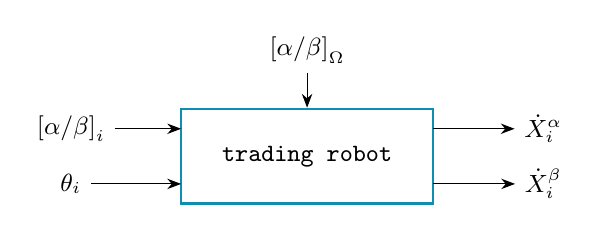
\begin{tikzpicture}[>={Stealth[length=5pt]}, font=\small]
        \node[draw=smoothblue, line width=1pt, minimum width=3.2cm, minimum height=1.2cm] (robot) {\texttt{trading robot}};
        \node (mp)    at (0,1.35)     {$\priceAB_\Omega$};
        \node (est)   at (-3.0,0.35)  {$\priceAB_i$};
        \node (theta) at (-3.0,-0.35) {$\theta_i$};
        \node (xa)    at (3.0,0.35)   {$\dot{X}_i^\alpha$};
        \node (xb)    at (3.0,-0.35)  {$\dot{X}_i^\beta$};
        \draw[->] (mp)        -- (robot.north);
        \draw[->] (est)       -- (-1.6,0.35);
        \draw[->] (theta)     -- (-1.6,-0.35);
        \draw[->] (1.6,0.35)  -- (xa);
        \draw[->] (1.6,-0.35) -- (xb);
    \end{tikzpicture}
    \end{center}
    \item \emph{No bias between assets.} The defining equations are invariant under swapping the two assets:
    \begin{equation*}
        \alpha \leftrightarrow \beta \,.
    \end{equation*}
\end{enumerate}

\textbf{Rational-trader principles} (each trading robot trades rationally according to its participant inputs):

Let $x_i := \priceAB_\Omega / \priceAB_i$ denote the ratio between the market price and participant $i$'s estimate:
\begin{enumerate}
    \setcounter{enumi}{4}
    \item \emph{Buy low.} When the market prices an asset below the participant's estimate, the participant is willing to buy that asset:
    \begin{equation*}
        x_i < 1 \;\Longrightarrow\; \dot{X}_i^\beta > 0 \ \left(\text{and } \dot{X}_i^\alpha < 0\right).
    \end{equation*}
    \item \emph{Sell high.} When the market prices it above the estimate, the participant is willing to sell it:
    \begin{equation*}
        x_i > 1 \;\Longrightarrow\; \dot{X}_i^\beta < 0 \ \left(\text{and } \dot{X}_i^\alpha > 0\right)\,.
    \end{equation*}
    At the estimate, they do not trade:
    \begin{equation*}
        x_i = 1 \;\Longrightarrow\; \dot{X}_i^\alpha = \dot{X}_i^\beta = 0\,.
    \end{equation*}
    \item \emph{Urgency grows with the gap.} Each exchange velocity varies strictly and monotonically with the gap between market price and estimate:
    \begin{equation*}
        \dot{X}_i^\alpha \ \text{is strictly increasing in } x_i \ \left(\text{and } \dot{X}_i^\beta \text{ strictly decreasing}\right),
    \end{equation*}
    so that $|\dot{X}_i^\alpha|$ and $|\dot{X}_i^\beta|$ grow as $x_i$ moves away from 1 in either direction.
    \item \emph{Urgency grows with confidence.} A participant's exchange velocities scale with a weight $w_i$ that increases strictly with their degree of confidence $\theta_i$:
    \begin{equation*}
        \dot{X}_i^\alpha\text{ and }\dot{X}_i^\beta\text{ are both }\propto w_i = w(\theta_i)\,, \quad w \ \text{strictly increasing in } \theta_i\,.
    \end{equation*}
    No conviction, no trade: $w(0) = 0$.
\end{enumerate}

These eight principles are the \emph{hypotheses} of the \StokEx{}: everything that follows is constructed to satisfy them. The symmetric exchange-velocity pair \eqref{eqExchangeSymmetry} realizes principles~2--4, the trader function \eqref{eqTraderFunction} realizes principles~5--7, the weight function \eqref{eqFunctionW} realizes principle~8, and finally the closed form of market price \eqref{eqMarketPrice} realizes principle~1.


% ----------------------------------------------------------------------
\section{Core Equations of the \StokEx{} Algorithm}
% ----------------------------------------------------------------------

\subsection{The personal trading robot} % locked
% ----------------------------------------------------------------------

Everything in this subsection is written from the point of view of a single participant, taking the market price $\priceAB_\Omega$ as a given input. We give the two exchange velocities that the participant's trading robot outputs, the profit it accumulates over time, the moment it empties an account, and a worked example on real data. The market price it reacts to is itself constructed, from the aggregate of all participants' trading robots, in Sec.~\ref{secMarketPrice}.

\subsubsection{Exchange-velocity function}
% ----------------------------------------------------------------------

Every participant in the \StokEx{} has their exchange velocities --- the output of their personal trading robot (Fig.~\ref{figRobotSchema}) --- determined by the same function. In that sense, the \StokEx{} fulfills principle number~3 (\emph{no bias between participants}).

This function requires two inputs from the participant:

\begin{tabularx}{\textwidth}{rX}
 $[\alpha/\beta]_i$ & participant $i$'s estimate of the value of 1~unit of~$\beta$ priced in~$\alpha$ \\
$\theta_i$ & participant $i$'s degree of confidence ($[0,100)\,\%$) in their estimate of the relative value of the two assets.
\end{tabularx}

\begin{figure}[tb]
\centering
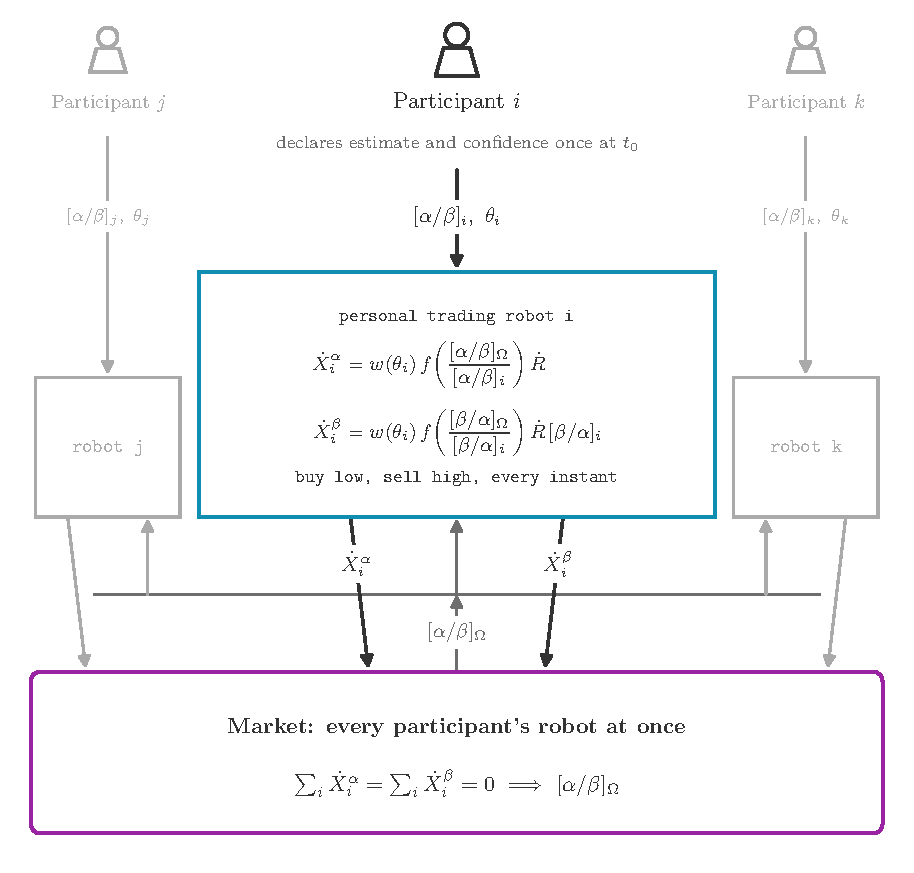
\includegraphics[width=0.75\textwidth]{personal_trading_robot.pdf}
\caption{General schema of a participant's personal trading robot: it takes the participant's own inputs and the current market price, and outputs the two exchange velocities. The single market price it reacts to emerges from the aggregate of every participant's robot at once and feeds back into each of them continuously. The same construction runs independently for every participant $i = 1, \dots, N$; three are shown here.}
\label{figRobotSchema}
\end{figure}

The function controlling the participant's exchange velocities in the \StokEx{} takes the following form:
\begin{align}
\dot{X}^\alpha_i &= w\!\left(\theta_i\right)\, f\!\left(\frac{\hspace{2pt}\priceAB_\Omega}{\priceAB_i} \right) \, \dot{R} \nonumber \, , \\
\dot{X}^\beta_i &=  w\!\left(\theta_i\right)\, f\!\left(\frac{\hspace{2pt}\priceBA_\Omega}{\priceBA_i} \right) \, \dot{R} \priceBA_i \,,
\label{eqExchangeSymmetry}
\end{align}
where $w$ is the weight function, $f$ is the trader function and $\dot{R}$ is the reference exchange velocity.

The reference exchange velocity $\dot{R}$ serves as a velocity unit (in $\alpha$ / unit of time), constant and common to all participants for this particular market. For example, in a market where gold is exchanged for dollars, the reference exchange velocity could be set to 1~dollar per second or 1~gram of gold per hour or whatever reference velocity makes sense in the context of that particular market. The asset in which $\dot{R}$ is denoted corresponds to asset A in this document. The corresponding reference exchange velocity for asset B is $\dot{R} \priceBA_i$ in the eyes of participant~$i$. For them, both $\dot{R}$ and $\dot{R} \priceBA_i$ are arbitrary yet consistent units of velocity. Importantly, the market price $\priceAB_\Omega$ does not depend on $\dot{R}$.

In effect, the two lines of \eqref{eqExchangeSymmetry} are one and the same equation, read once with $\alpha$ and once with $\beta$ and it respects the symmetry of principle principle number~4 (\emph{no bias between assets}), as we show in Annex~\ref{secReferenceVelocityBias}. Next, we need to specify the functions~$w$ and~$f$ that compose the exchange-velocity function.

\clearpage
\subsubsection{The trader function}
% ----------------------------------------------------------------------

Let us first define the \emph{trader function}~$f$. It maps a single variable --- the ratio between the market price and a participant's estimate, either $\priceAB_\Omega / \priceAB_i$ or $\priceBA_\Omega / \priceBA_i$ --- onto the normalized behavior that every personal trading robot shares.

This common behavior follows principles number~5, 6 and~7 (\emph{buy low}, \emph{sell high}, \emph{urgency grows with the gap}). The \StokEx{} satisfies these principles by defining the trader function, for any price ratio $x > 0$, as
\begin{equation}
    f(x) = x^2 - \frac{1}{x}\,. \label{eqTraderFunction}
\end{equation}
Figure~\ref{figTraderFunction} shows it.

This choice is principled but not arbitrary. As shown in Annex~\ref{secTraderFamily}, principles 2 and 4 (\emph{exchange at market price} and \emph{no bias between assets}) by themselves force two structural properties of any admissible trader function: the functional equation $f(1/x) = -f(x)/x$, and hence $f(1) = 0$ (no trade at one's own estimate). The functions compatible with all eight principles and with a closed-form market price form a one-parameter family, of which \eqref{eqTraderFunction} is the minimal member with unbounded urgency on both the buying and the selling side; the whole family is described in Annex~\ref{secTraderFamily} and is part of the present disclosure.

\begin{figure}[tb]
\centering
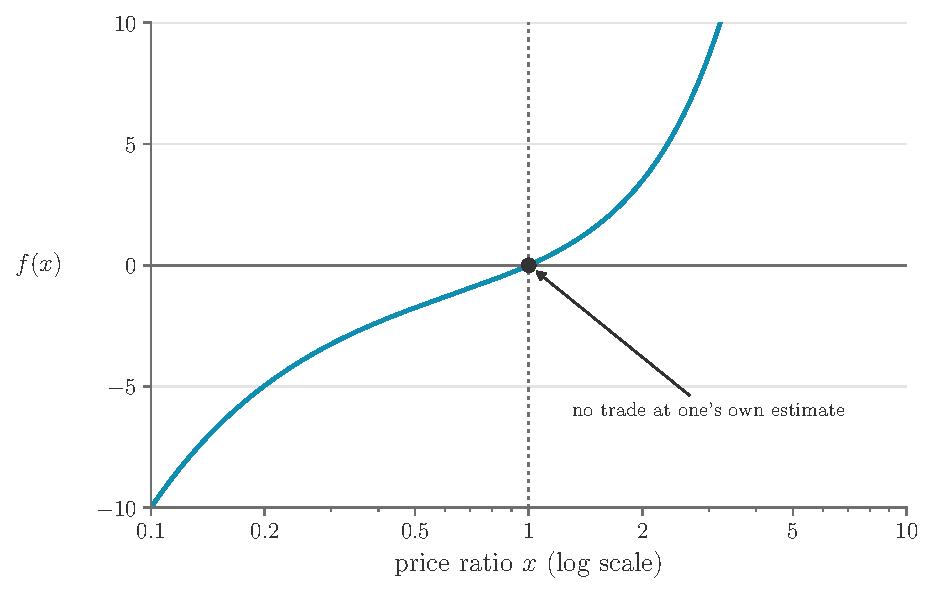
\includegraphics[width=0.75\textwidth]{trader_function.pdf}
\caption{The trader function $f(x) = x^2 - 1/x$, where $x$ is the ratio between the market price and the participant's own estimate. It vanishes at $x = 1$ (no trade at one's own estimate), is negative below it and positive above it, and grows without bound on both sides: the further the market strays from the estimate, the more urgent the trade.}
\label{figTraderFunction}
\end{figure}

\textbf{Numerical evaluation of the trader function}:

Each robot evaluates the trader function at the ratio between the market price and its participant's estimate:
\begin{align}
f_i^\alpha &:= f\!\left(\frac{\hspace{2pt}\priceAB_\Omega}{\priceAB_i} \right)\, , \nonumber \\
f_i^\beta &:= f\!\left(\frac{\hspace{2pt}\priceBA_\Omega}{\priceBA_i} \right) \, .
\label{eqFunctionX}
\end{align}

The typical operating point of the \StokEx{} is $x \approx 1$: participants' estimates hover around the market price. Precisely there, the defining expression $f(x) = x^2 - 1/x$ suffers \emph{catastrophic cancellation} in floating-point arithmetic: both terms are close to 1, and their subtraction erases up to half of the significand. Measured against exact rational arithmetic (IEEE-754 double precision), the relative error of the standard form reaches $4 \times 10^{-2}$ at $x = 1 - 10^{-15}$.

The remedy is the \emph{shifted form}. Let $y = x - 1$; for $x \in [1/2,\ 2]$ this subtraction is exact in floating point (Sterbenz's lemma), and $x^3 - 1 = y^3 + 3y^2 + 3y$, so that
\begin{equation}
    f(x) = \frac{y\left(y^2 + 3y + 3\right)}{x}\,, \qquad y = x - 1\,. \label{eqShiftedForm}
\end{equation}
The numerator tracks the small deviation $y$ directly, without cancellation, and the denominator must be the \emph{input} $x$ itself: recomputing it as $y + 1$ reintroduces a relative error that grows toward the ends of the domain, up to $\sim 10^{-5}$ at $x = 10^{-12}$. The expression is branchless (no conditional jumps), constant-time (a straight line of fused multiply-adds --- \emph{fma}) and its measured relative error stays below $6 \times 10^{-16}$ (machine precision) over $x \in [10^{-12},\ 10^{12}]$. This domain is wider than the price bounds of the reference implementation: estimates are bounded to $[10^{-6},\ 10^{6}]$ and the market price always lies between the smallest and the largest estimate (see the corollary in Annex~\ref{secProofUniqueness}), so the \emph{ratio} of the two spans up to twelve decades on each side of 1.


\subsubsection{The weight function}
% ----------------------------------------------------------------------

Second, we define the function $w$ that serves as a weighting factor for each participant in the \StokEx{}. It maps a participant's degree of confidence $[0, 100)\,\%$ onto $[0,+\infty)$, such that
\begin{equation}
    w_i := w\left(\theta_i\right) = \frac{1}{3}\tan \left( \frac{\pi \,\theta_i}{200\%}\right)\,. \label{eqFunctionW}
\end{equation}
The function $w$ is consistent with principle number 8 (\emph{urgency grows with confidence}) since it scales the participant's exchange velocities according to their degree of confidence. In Fig.~\ref{figDegreeBoth}, we show that $\theta_i$ can be interpreted as a geometrical angle in the right context (see proof in Annex \ref{secProofDegree}). This tangent map is a design choice, not a requirement: principle 8 (\emph{urgency grows with confidence}) only asks for a strictly increasing $w$ with $w(0) = 0$, and Annex~\ref{secWeightFamily} shows that every result in this document holds unchanged for any such function.

The participant's weight $w_i$ is computed once at the beginning of the algorithm and it remains constant until the participant revises their degree of confidence $\theta_i$.

\begin{figure}[hb]
    \centering
    \begin{subfigure}[t]{0.48\textwidth}
        \centering
        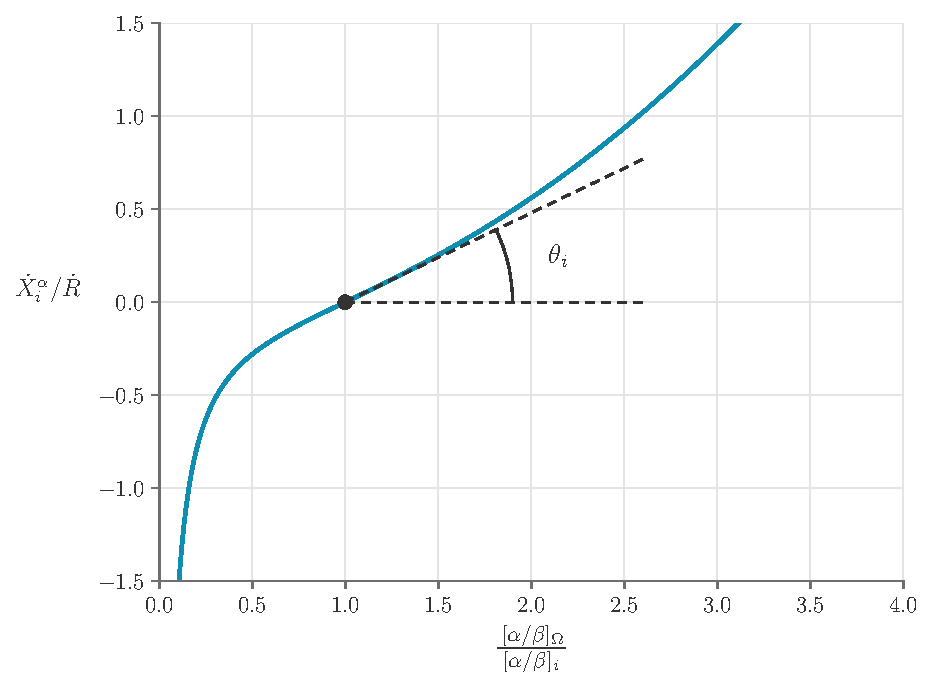
\includegraphics[width=\textwidth]{degree_of_certainty.pdf}
        \caption{Linear scale in $x$}
        \label{figDegree}
    \end{subfigure}
    \hfill
    \begin{subfigure}[t]{0.48\textwidth}
        \centering
        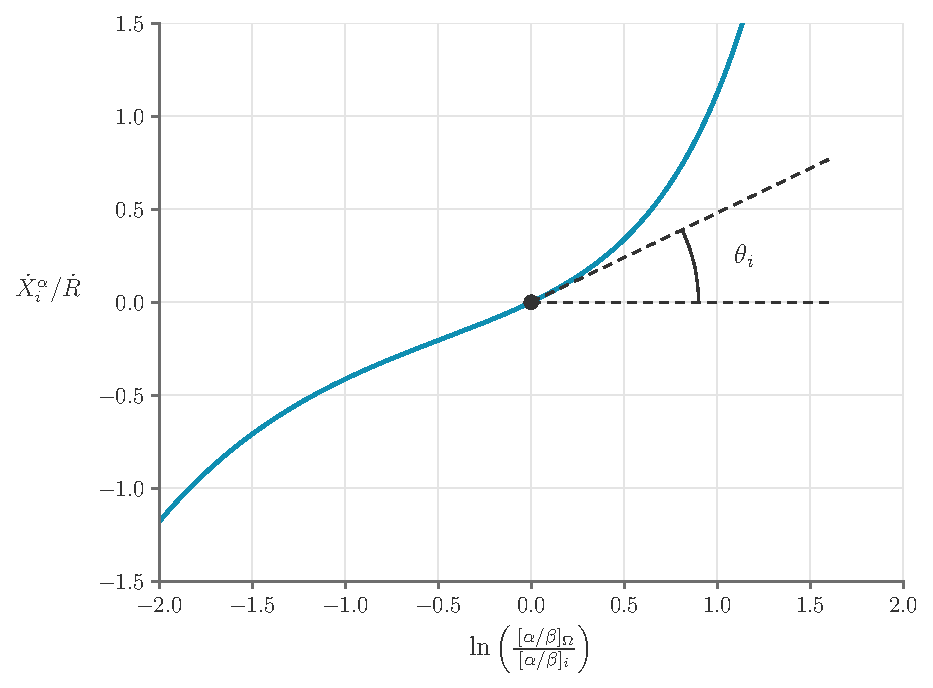
\includegraphics[width=\textwidth]{degree_of_certainty_log.pdf}
        \caption{Logarithmic scale in $x$}
        \label{figDegreeLog}
    \end{subfigure}
    \caption{Geometrical interpretation of the participant's degree of confidence $\theta_i$}
    \label{figDegreeBoth}
\end{figure}


\clearpage
\subsubsection{Consistency with the principles}
% ----------------------------------------------------------------------

Thus, the algebraic equations for the exchange velocities of participant $i$ are
\begin{align}
    \dot{X}^\alpha_i &= w_i \left( \left( \frac{\hspace{2pt}\priceAB_\Omega}{\priceAB_i}\right)^2 - \frac{\priceAB_i}{\hspace{2pt}\priceAB_\Omega} \right) \dot{R}\,, \nonumber\\
    \dot{X}^\beta_i &= w_i \left( \left( \frac{\hspace{2pt}\priceBA_\Omega}{\priceBA_i}\right)^2 - \frac{\priceBA_i}{\hspace{2pt}\priceBA_\Omega} \right) \dot{R} \priceBA_i\,. \label{eqExchangeVelocities}
\end{align}


In Fig.~\ref{figExchangeSymmetry}, we can see that, expressed in the same units of $\dot{R}$, the two curves are mirror images of one another (unbiased toward one asset or the other) and that they allow each participant to automatically ``buy low and sell high'' according to their estimate of the relative value of assets~A and~B.

\begin{figure}[tb]
\centering
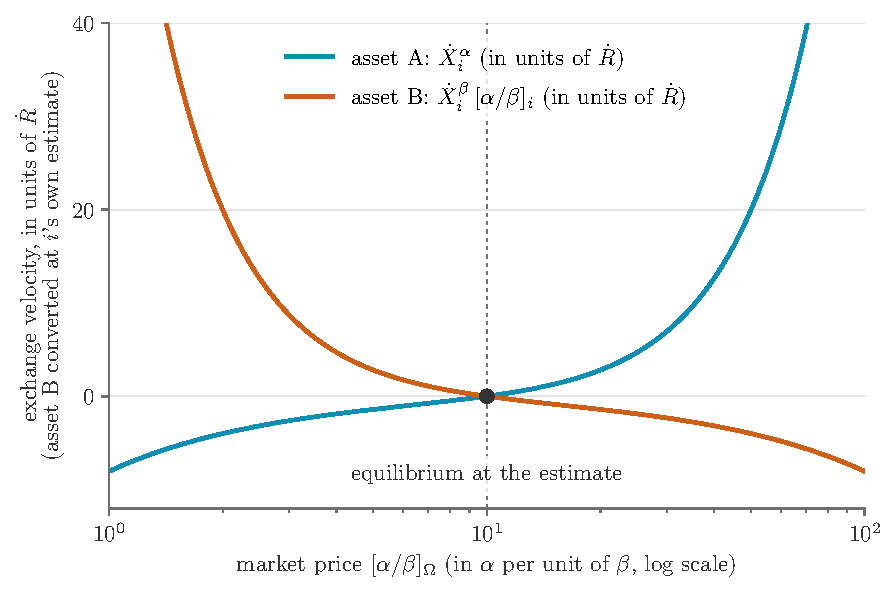
\includegraphics[width=0.75\textwidth]{stokex_symmetry.pdf}
\caption{participant $i$'s exchange velocities for an estimate of $\priceAB_i = 10$~$\alpha$ per~$\beta$ with a degree of confidence $\theta_i= 75 \%$. To compare both exchange velocities on a single axis, asset~B's velocity is converted to its $\alpha$-equivalent using the participant's own estimate, $\dot{X}_i^\beta \priceAB_i$ --- the fair conversion factor according to participant $i$, not the (generally different) market price $\priceAB_\Omega$.}
\label{figExchangeSymmetry}
\end{figure}

In Annex \ref{secProofExchangeAtMarketPrice}, we prove that the expressions in \eqref{eqExchangeVelocities} are consistent with principle number~2 (\emph{exchange at market price}). Formally, this means that
\begin{equation}\label{eqExchangeAtMarketPrice}
    \left[\alpha/\beta\right]_\Omega = - \frac{\dot{X}^\alpha_i}{\dot{X}^\beta_i} \,.
\end{equation}
Indeed, if a participant is buying asset A and paying with asset B, the two exchange velocities must be of opposite sign and the proportionality constant between the two is the market price. In Sec.~\ref{secMarketPrice}, we will determine the expression to compute the market price $\priceAB_\Omega$.

\clearpage
\subsubsection{Time it takes to empty a participant's account}
% ----------------------------------------------------------------------

With the participant's exchange velocities, we can predict when each of their two account balances reaches zero. As long as the state of the market is constant, each balance changes linearly. Only the account of a sold asset ever empties: the ratio $-n_i/\dot{X}_i$ is a positive time when that asset's velocity is negative, but a meaningless negative number for an asset that is being bought. We therefore set the emptying time of an account to that ratio when its asset is being sold, and to $+\infty$ otherwise:
\begin{align}
    \Delta t_i^\alpha &= \begin{cases} -\, n_i^\alpha / \dot{X}_i^\alpha \,, & \dot{X}_i^\alpha < 0 \,,\\ +\infty \,, & \dot{X}_i^\alpha \geq 0 \,, \end{cases} \nonumber\\
    \Delta t_i^\beta &= \begin{cases} -\, n_i^\beta / \dot{X}_i^\beta \,, & \dot{X}_i^\beta < 0 \,,\\ +\infty \,, & \dot{X}_i^\beta \geq 0 \,. \end{cases} \label{eqDeltaT}
\end{align}
Because the two velocities always carry opposite signs (principle~2, \emph{exchange at market price}), at most one of $\Delta t_i^\alpha$ and $\Delta t_i^\beta$ is finite --- that of the asset currently being sold. The participant's emptying time is therefore
\begin{equation}
    \Delta t_i = \min\!\left(\Delta t_i^\alpha,\, \Delta t_i^\beta\right) \,,
\end{equation}
which returns exactly that account; it is $+\infty$ only when the market matches the participant's estimate, so that neither asset trades. The $+\infty$ convention is what lets the minimum select the right account: without it, the negative raw ratio of the bought account would spuriously win.

\subsubsection{Participant's profit over a given time period}\label{secParticipantProfit}
% ----------------------------------------------

Relative to an arbitrary reference time $t_0$ (e.g.\ when the participant joined the market, or any other point of interest), participant $i$'s profit since $t_0$ is obtained by marking the change in \emph{both} balances to market at today's price, in either asset:
\begin{align}
    P_i^\alpha(t) &= \left(n_i^\alpha(t) - n_i^\alpha(t_0)\right) + \left(n_i^\beta(t) - n_i^\beta(t_0)\right)\priceAB_\Omega\!(t) \,, \label{eqParticipantProfitAlpha}\\
    P_i^\beta(t) &= \left(n_i^\beta(t) - n_i^\beta(t_0)\right) + \left(n_i^\alpha(t) - n_i^\alpha(t_0)\right)\priceBA_\Omega\!(t) \,. \label{eqParticipantProfitBeta}
\end{align}
By construction $P_i^\alpha(t_0) = 0\,\alpha$ and $P_i^\beta(t_0) = 0\,\beta$: there is no profit relative to itself. Using $\priceBA_\Omega = 1/\priceAB_\Omega$, the two quantities satisfy
\begin{equation}
    P_i^\alpha(t) = P_i^\beta(t)\, \priceAB_\Omega(t) \,. \label{eqProfitIdentity}
\end{equation}
Profit is therefore never independent of the asset it is quoted in: it is not that one of $P_i^\alpha$ and $P_i^\beta$ is ``the'' profit and the other a unit conversion of it, but that both are equally valid, related exactly by the market price of the moment. Because that price is always strictly positive (principle 2, \emph{exchange at market price}), $P_i^\alpha(t)$ and $P_i^\beta(t)$ always agree in sign --- a participant cannot be ahead in one asset and behind in the other --- but they generally disagree in magnitude, by exactly the factor $\priceAB_\Omega(t)$. This is the \StokEx{}'s asset symmetry (principle 4, \emph{no bias between assets}) carried into the derived notion of profit: no asset is privileged as the numeraire in which profit must be reported.


\subsubsection{Numerical illustration: a currency pair (CAD/EUR)}
% ----------------------------------------------------------------------

This subsection shows a single personal trading robot in action, with a fictional participant but real market data. Only the exchange-velocity function \eqref{eqExchangeVelocities} is at work here: the real exchange rate is handed to the robot from the outside, instead of emerging from the other participants as it would in the full \StokEx{} algorithm.

\begin{figure}[htbp]
\centering
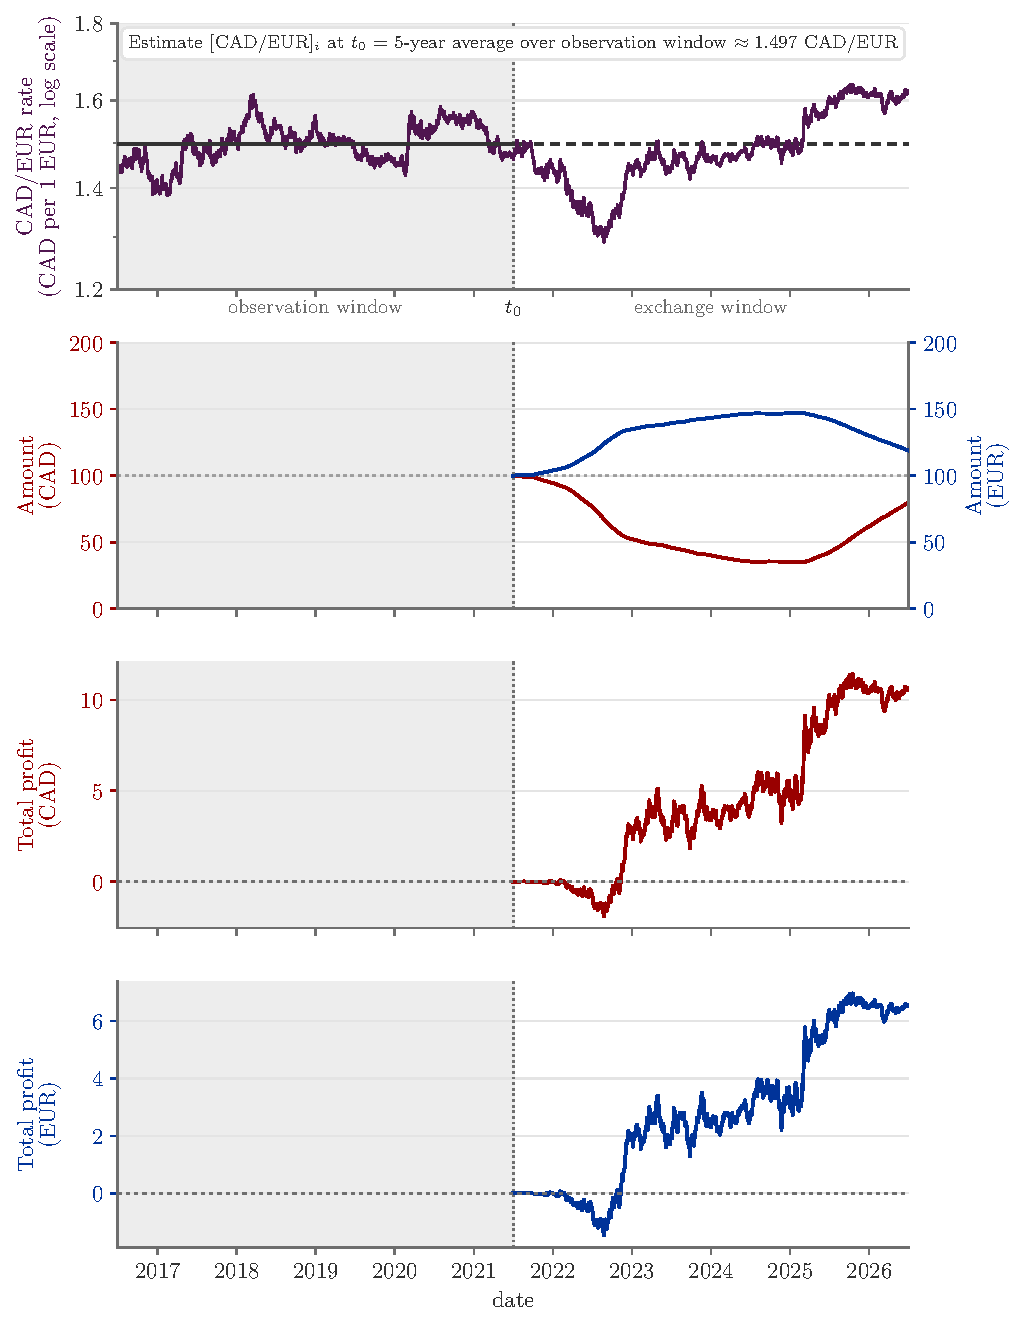
\includegraphics[width=0.85\textwidth]{cadeur_example.pdf}
\caption{Numerical illustration on real data: the CAD/EUR exchange rate (top, FRED series \texttt{DEXCAUS}~\cite{FREDDEXCAUS} and \texttt{DEXUSEU}~\cite{FREDDEXUSEU}, price on a log axis) over the shaded observation window, 2016-07-01 to 2021-07-01, used only to compute a plain average (solid, horizontal: no trend fit is warranted here) that becomes the declared estimate throughout the unshaded exchange window, 2021-07-01 to 2026-07-01, $\approx1.497$~CAD per EUR (dashed line). Second: the two account balances of Alice's wallet, starting at 100~CAD (red, left axis) and 100~EUR (blue, right axis), each kept in its own native currency. Third and fourth: Alice's profit since the start of the exchange window (Eqs.~\eqref{eqParticipantProfitAlpha}--\eqref{eqParticipantProfitBeta}), accounted in CAD ($P^{\mathrm{CAD}}$, red) and independently in EUR ($P^{\mathrm{EUR}}$, blue) --- the same quantity, related exactly by Eq.~\eqref{eqProfitIdentity}, not two independent findings.}
\label{figCADEURExample}
\end{figure}

It's July 1\textsuperscript{st} 2021. Alice holds dual Canadian and French citizenship, and keeps two accounts, one in Canadian dollars (CAD) and one in euros (EUR), with a small reserve in each --- 100~CAD and 100~EUR. At some time in the future, she may need to use that reserve in one country or the other and she will have to convert her entire reserve in either CAD or EUR. In the meantime, she wants to buy each currency while it is cheap and sell it while it is dear, continuously, without watching the rate all day. This is exactly what the personal trading robot of the \StokEx{} does for her.

As we have seen, Alice needs to answer two questions to deploy her personal trading robot on the CAD/EUR exchange: $\left.1\right)$ what she thinks one EUR is worth in CAD, and $\left.2\right)$ how confident she is in that estimate. Looking at the history of the CAD/EUR exchange rate data over the last 5 years (from July 1\textsuperscript{st} 2016 to 2021), she sees that the trend is pretty flat, so she makes her estimate at the average price over that 5-year window, which happens to be $\approx1.497$~CAD per EUR. She puts her degree of confidence at 70\%. This sets up her personal trading robot, which trades gently and continuously on her behalf. In Fig.~\ref{figCADEURExample} we show what that robot would have done over the next five years (from July 1\textsuperscript{st} 2021 to 2026) of real market data.

Over the exchange window Alice ends $\approx10.6$~CAD ($\approx6.5$~EUR) ahead: against a starting wealth of $\approx247$~CAD ($\approx168$~EUR), a five-year return of about 4\% (4.3\% counted in CAD, 3.9\% in EUR). The two profit curves are related exactly by \eqref{eqProfitIdentity}. Therefore ``How much richer is Alice'' is only a well-posed question once a currency is chosen to measure it in, and the \StokEx{} itself never makes that choice: every principle is stated in terms of exchange velocities and ratios, never in terms of a profit computed in one privileged asset.

\emph{A note on the reference exchange velocity.} Alice's robot's exchange velocities \eqref{eqExchangeVelocities} are both scaled by $\dot{R}$, the reference exchange velocity of this market. In the \tok{} system it has a natural value, the system's universal-income velocity (Sec.~\ref{secReferenceImplementation}); between two floating currencies there is no such anchor, because fiat money is not a stable unit of value --- the purchasing power of each drifts downward, at its own inflation rate, which no issuer commits to in advance. We therefore set $\dot{R} = 1$~CAD/day throughout, an arbitrary placeholder rather than an estimate of how actively a real participant trades: every CAD and EUR amount above is exactly proportional to it,while the fractions of days spent buying versus selling, and the dates of the largest signals, do not depend on it.

\subsection{The market}\label{secMarketPrice}
% ----------------------------------------------------------------------

As stated in principle number 1 (\emph{equilibrium and conservation}), the market price is the relative value that leads to an equilibrium between supply and demand. Formally, this means that the market price must satisfy
\begin{equation}
    \sum_i \dot{X}_i^\alpha = \sum_i \dot{X}_i^\beta = 0 \,. \label{eqEquilibrium}
\end{equation}
Indeed, at any given time and for both assets, the total amount being sold by some participants must be bought by some others: the \StokEx{} creates and destroys nothing, it only transfers.

Since the behavior of each participant is set in a rational way by \eqref{eqExchangeVelocities} and entirely defined by their two inputs $\priceAB_i$ and $\theta_i$, we find (see proof in Annex \ref{secProofMarketprice}) that the expression for the market price is
\begin{equation}
    \priceAB_\Omega = \left( \frac{\displaystyle \sum_i w_i \priceAB_i}{\displaystyle \sum_i w_i \priceBA_i^2}\right)^{1/3}\,. \label{eqMarketPrice}
\end{equation}
In this expression, the sum over the participants only includes those who are actually able to trade (i.e. they have the asset they wish to sell).

Let us note that this equilibrium price is \emph{unique}: by principle 7 (\emph{urgency grows with the gap}), each participant's exchange velocity is strictly increasing in the market price, hence so is the net exchange velocity $\sum_i \dot{X}_i^\alpha$, so it can vanish at only one strictly positive price, the one given by \eqref{eqMarketPrice}. The precise conditions and the proof are given in Annex~\ref{secProofUniqueness}.

\clearpage
% ----------------------------------------------------------------------
\section{Implementation of the \StokEx{} Algorithm}
% ----------------------------------------------------------------------

The equations of the \StokEx{} that were developed in the previous section are valid as long as both inputs from all participants remain constant and as long as each participant has a positive balance in the account holding the asset they are selling. Of course, at some point in time, these conditions are bound to change. Therefore, the \StokEx{} operates in steps during which the state of the market remains constant (i.e. constant market price and constant exchange velocities).

In general, we know the balance of every account at $t_0$ and we want to know their balance at $t_1$, when a participant requests an action. The actions available to the participant are:
\begin{enumerate}
    \item check the market price,
    \item check their account balance,
    \item deposit/withdraw an amount,
    \item change their estimate or degree of confidence.
\end{enumerate}

Between $t_0$ and $t_1$, both inputs from all participants are constant. However, we must automatically handle the cases when one of the participants runs out of the asset they are selling between $t_0$ and $t_1$. Each time this happens, the state of the market must be updated.

Thus, the \StokEx{} is implemented in two parts. First we describe the inner algorithm responsible for outputting the current state of the market. Second we describe the outer algorithm that performs the time stepping to get from $t_0$ to $t_1$. This process is illustrated in Fig.~\ref{figMarketSteps}.

\begin{figure}[htbp]
\centering
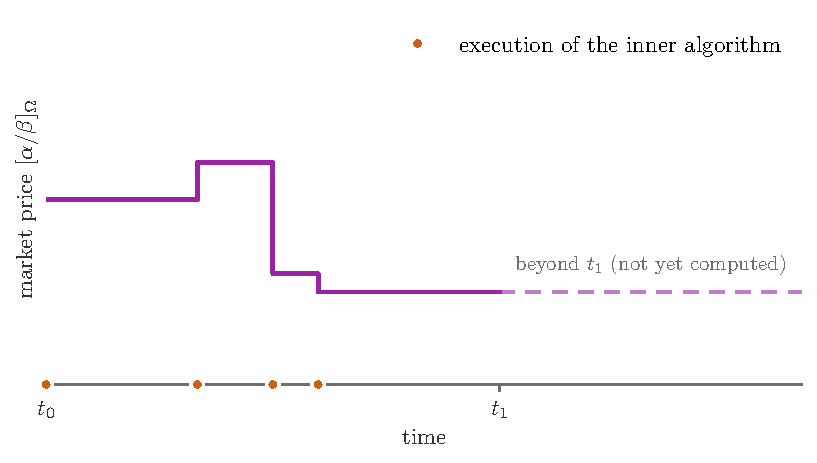
\includegraphics[width=0.75\textwidth]{stokex_steps.pdf}
\caption{Process by which the state of the \StokEx{} is updated between $t_0$ and $t_1$.}
\label{figMarketSteps}
\end{figure}
\clearpage

\subsection{Inner \StokEx{} Algorithm}
% ----------------------------------------------------------------------

The purpose of the inner algorithm is to return the market price and participants' exchange velocities at the current time $t$. The inner algorithm takes into account that some participants might have run out of the asset they wish to sell. These participants must therefore be excluded from the market since their estimate is irrelevant. By excluded from the market, we mean that both their exchange velocities are zero and that their input parameters are not taken into account for the computation of the market price.

When a participant runs out of the asset they are selling, they are automatically excluded from the market. On the other hand, when the excluded participants are in a situation where they can participate again, they are also automatically reintegrated in the market.

\subsubsection{Inputs}
Each participant in the market must provide the following information:

\begin{tabularx}{\textwidth}{rX}
 $[\alpha/\beta]_i$ & participant $i$'s estimate of the value of 1 unit of $\beta$ priced in $\alpha$ \\
$\theta_i$ & participant $i$'s degree of confidence ($[0,100)\,\%$) in their estimate of the relative value of the two assets.
\end{tabularx}

In addition, we must provide to the algorithm the balance for both accounts of every participant at the current time $t$:

\begin{tabularx}{\textwidth}{rX}
 $n_i^\alpha$ & participant $i$'s balance of asset A (in $\alpha$) \\
$n_i^\beta$ & participant $i$'s balance of asset B (in $\beta$)
\end{tabularx}

\subsubsection{Outputs}
From the above inputs, the algorithm calculates and returns the following information:

\begin{tabularx}{\textwidth}{rX}
 $[\alpha/\beta]_\Omega$ & The market price of 1 unit of $\beta$ priced in $\alpha$ \\
$\dot{X}^\alpha_i$ & participant $i$'s exchange velocity of asset A (in $\alpha$ per unit of time)\\
$\dot{X}^\beta_i$ & participant $i$'s exchange velocity of asset B (in $\beta$ per unit of time) \\
$\Delta t_i$ & the amount of time after which participant $i$ runs out of the asset they are selling
\end{tabularx}

\subsubsection{Plain description of the inner \StokEx{} algorithm}
\begin{itemize}
    \item Exclude every participant that has at least one empty account from the market and add them to a checklist. (lines 3-10)
    \item Compute the market price using \eqref{eqMarketPrice}. (line 11)
    \item For each participant that has been excluded, check if they have a positive balance in the account holding the asset they wish to sell. If so, reintegrate them in the market and compute the new market price using \eqref{eqMarketPrice}. Once a participant has been checked, remove them from the checklist. Repeat this process until no participant is left on the checklist. Since reintegrating a participant in the market changes the market price, we have to be careful with the order in which we cross off the participants from the checklist. To ensure that this process is done properly, it can be shown that we must always check the participant whose value estimate is the ``furthest'' away from the market price, our metric for the distance being $|f_i^\alpha|$, computed using \eqref{eqFunctionX}. To find that participant efficiently, the checklist is first \emph{sorted} by estimate. For any given price, since $f$ is monotone in the estimate, the largest $|f_i^\alpha|$ is always attained at one of the two ends of the sorted checklist, so each step examines two participants only. Each reintegration then updates the market price in $O(1)$: the participant's terms are added to the two market sums of \eqref{eqMarketPrice} and the price is recomputed from them (the same incremental bookkeeping as the market update of Sec.~\ref{secMarketUpdate}). (lines 12-21)
    \item For each participant, compute their exchange velocities, using \eqref{eqExchangeVelocities}, and the time it will take to empty the account for the asset they are selling, using \eqref{eqDeltaT}. (lines 22-36)
\end{itemize}

\subsubsection{Pseudocode for the inner \StokEx{} algorithm}
\begin{algorithmic}[1]
    \STATE \textbf{given} the account balance $n_i^\alpha$ and $n_i^\beta$ for every participant
    \STATE \textbf{given} the inputs $\priceAB_i$ and $\theta_i$ for every participant
    \FORALL{participants}
        \IF{$n_i^\alpha = 0$ \OR $n_i^\beta = 0$}
            \STATE exclude participant $i$ from the market
            \STATE add participant $i$ to checklist
        \ELSE
            \STATE include participant $i$ in the market
        \ENDIF
    \ENDFOR
    \STATE compute $\priceAB_\Omega$
    \STATE sort the checklist by increasing estimate $\priceAB_i$
    \WHILE{checklist is not empty}
        \STATE compute $f^\alpha$ at both ends of the checklist
        \STATE $i^{\ast} \gets$ the end with the largest $|f^\alpha|$
        \IF{($f_{i^{\ast}}^\alpha \geq 0$ \AND $n_{i^{\ast}}^\beta > 0$) \OR ($f_{i^{\ast}}^\alpha \leq 0$ \AND $n_{i^{\ast}}^\alpha > 0$)}
            \STATE include participant $i^{\ast}$ in the market
            \STATE update $\priceAB_\Omega$ incrementally
        \ENDIF
        \STATE remove participant $i^{\ast}$ from checklist
    \ENDWHILE
    \FORALL{participants}
        \IF{participant $i$ is included in the market}
            \STATE compute $\dot{X}_i^\alpha$ and $\dot{X}_i^\beta$
        \ELSE
            \STATE $\dot{X}_i^\alpha \gets 0$ and $\dot{X}_i^\beta \gets 0$
        \ENDIF
        \IF{$\dot{X}_i^\alpha < 0$}
            \STATE $\Delta t_i \gets - n_i^\alpha / \dot{X}_i^\alpha$
        \ELSIF{$\dot{X}_i^\beta < 0$}
            \STATE $\Delta t_i \gets - n_i^\beta / \dot{X}_i^\beta$
        \ELSE
            \STATE $\Delta t_i \gets +\infty$
        \ENDIF
    \ENDFOR
    \RETURN $\priceAB_\Omega$, $\dot{X}_i^\alpha$, $\dot{X}_i^\beta$ and $\Delta t_i$
\end{algorithmic}

\textbf{Complexity.} The exclusion pass, the from-scratch market price and the final velocity computation are all $O(N)$; the checklist sort is $O(N \log N)$; each reintegration step costs $O(1)$ thanks to the incremental update of the two market sums. The inner \StokEx{} algorithm therefore runs in $O(N \log N)$ overall.
\clearpage


\subsection{Outer \StokEx{} Algorithm}
% ----------------------------------------------------------------------

The outer algorithm performs the necessary time steps to get from $t_0$ to $t_1$. If a participant runs out of the asset they are selling during that time interval, the outer algorithm steps up to that instant to update the state of the market. This process repeats until $t_1$ is reached.

\subsubsection{Inputs}

\begin{tabularx}{\textwidth}{rX}
 $t_0$ & Initial time \\
$t_1$ & Final time
\end{tabularx}

Each participant in the market must provide the following information:

\begin{tabularx}{\textwidth}{rX}
 $[\alpha/\beta]_i$ & participant $i$'s estimate of the value of 1 unit of $\beta$ priced in $\alpha$ \\
$\theta_i$ & participant $i$'s degree of confidence ($[0,100)\,\%$) in their estimate of the relative value of the two assets.
\end{tabularx}

In addition, we must provide to the algorithm the balance for both accounts of every participant at the initial time $t_0$:

\begin{tabularx}{\textwidth}{rX}
 $n_i^\alpha$ & participant $i$'s balance of asset A (in $\alpha$) \\
$n_i^\beta$ & participant $i$'s balance of asset B (in $\beta$)
\end{tabularx}

\subsubsection{Outputs}
From the above inputs, the algorithm calculates and returns the market price and the balance for both accounts of every participant at $t_1$:

\begin{tabularx}{\textwidth}{rX}
 $[\alpha/\beta]_\Omega$ & The market price of 1 unit of $\beta$ priced in $\alpha$ \\
 $n_i^\alpha$ & participant $i$'s balance of asset A (in $\alpha$) \\
$n_i^\beta$ & participant $i$'s balance of asset B (in $\beta$)
\end{tabularx}

\subsubsection{Pseudocode for the outer \StokEx{} algorithm}

\begin{algorithmic}[1]
    \STATE \textbf{given} an initial time $t_0$
    \STATE \textbf{given} a final time $t_1$
    \STATE \textbf{given} the account balances $n_i^\alpha$ and $n_i^\beta$ for every participant (at $t_0$)
    \STATE \textbf{given} the inputs $\priceAB_i$ and $\theta_i$ for every participant (constant between $t_0$ and $t_1$)
    \STATE $t \gets t_0$
    \STATE \textbf{execute} inner \StokEx{} algorithm
    \STATE $\Delta t \gets \min_i \Delta t_i$
    \WHILE{$t_1 - t \geq \Delta t$}
        \FORALL{participants}
            \STATE $n_i^\alpha \gets n_i^\alpha + \dot{X}_i^\alpha \Delta t$
            \STATE $n_i^\beta \gets n_i^\beta + \dot{X}_i^\beta \Delta t$
        \ENDFOR
        \STATE $t \gets t + \Delta t$
        \STATE \textbf{execute} inner \StokEx{} algorithm
        \STATE $\Delta t \gets \min_i \Delta t_i$
    \ENDWHILE
    \STATE $\Delta t \gets t_1 - t$
    \FORALL{participants}
        \STATE $n_i^\alpha \gets n_i^\alpha + \dot{X}_i^\alpha \Delta t$
        \STATE $n_i^\beta \gets n_i^\beta + \dot{X}_i^\beta \Delta t$
    \ENDFOR
    \RETURN $n_i^\alpha$, $n_i^\beta$ and $\priceAB_\Omega$ (at $t_1$)
\end{algorithmic}

\subsection{Reference implementation in the \tok{} system}\label{secReferenceImplementation}
% ----------------------------------------------------------------------

In the \tok{} system, the \StokEx{} is instantiated with $\alpha$ = the \tok{} (a universal-income-based currency with continuous exponential disintegration) and $\beta$ = a foreign currency (CAD, EUR, \ldots), with one market per foreign currency. The reference implementation uses the following parameters: the reference exchange velocity $\dot{R}$ is set to the universal income velocity of the \tok{} system (1~\tok{} per 15~days); estimates are bounded to $10^{-6} \leq \priceAB_i \leq 10^{6}$; degrees of confidence are discretized with a step of $10^{-4}\,\%$ and capped at $99.9999\,\%$; the default market price of an empty market is 1.

Figure~\ref{figRefImplUI} shows this interface in operation, with the \tok{} exchanged against a fictional foreign currency, the TIK: a participant reads off the current market rate and their two balances, and declares the two inputs --- an estimate of the relative value and a degree of confidence --- from which their personal trading robot is set up.

\begin{figure}[htbp]
\centering
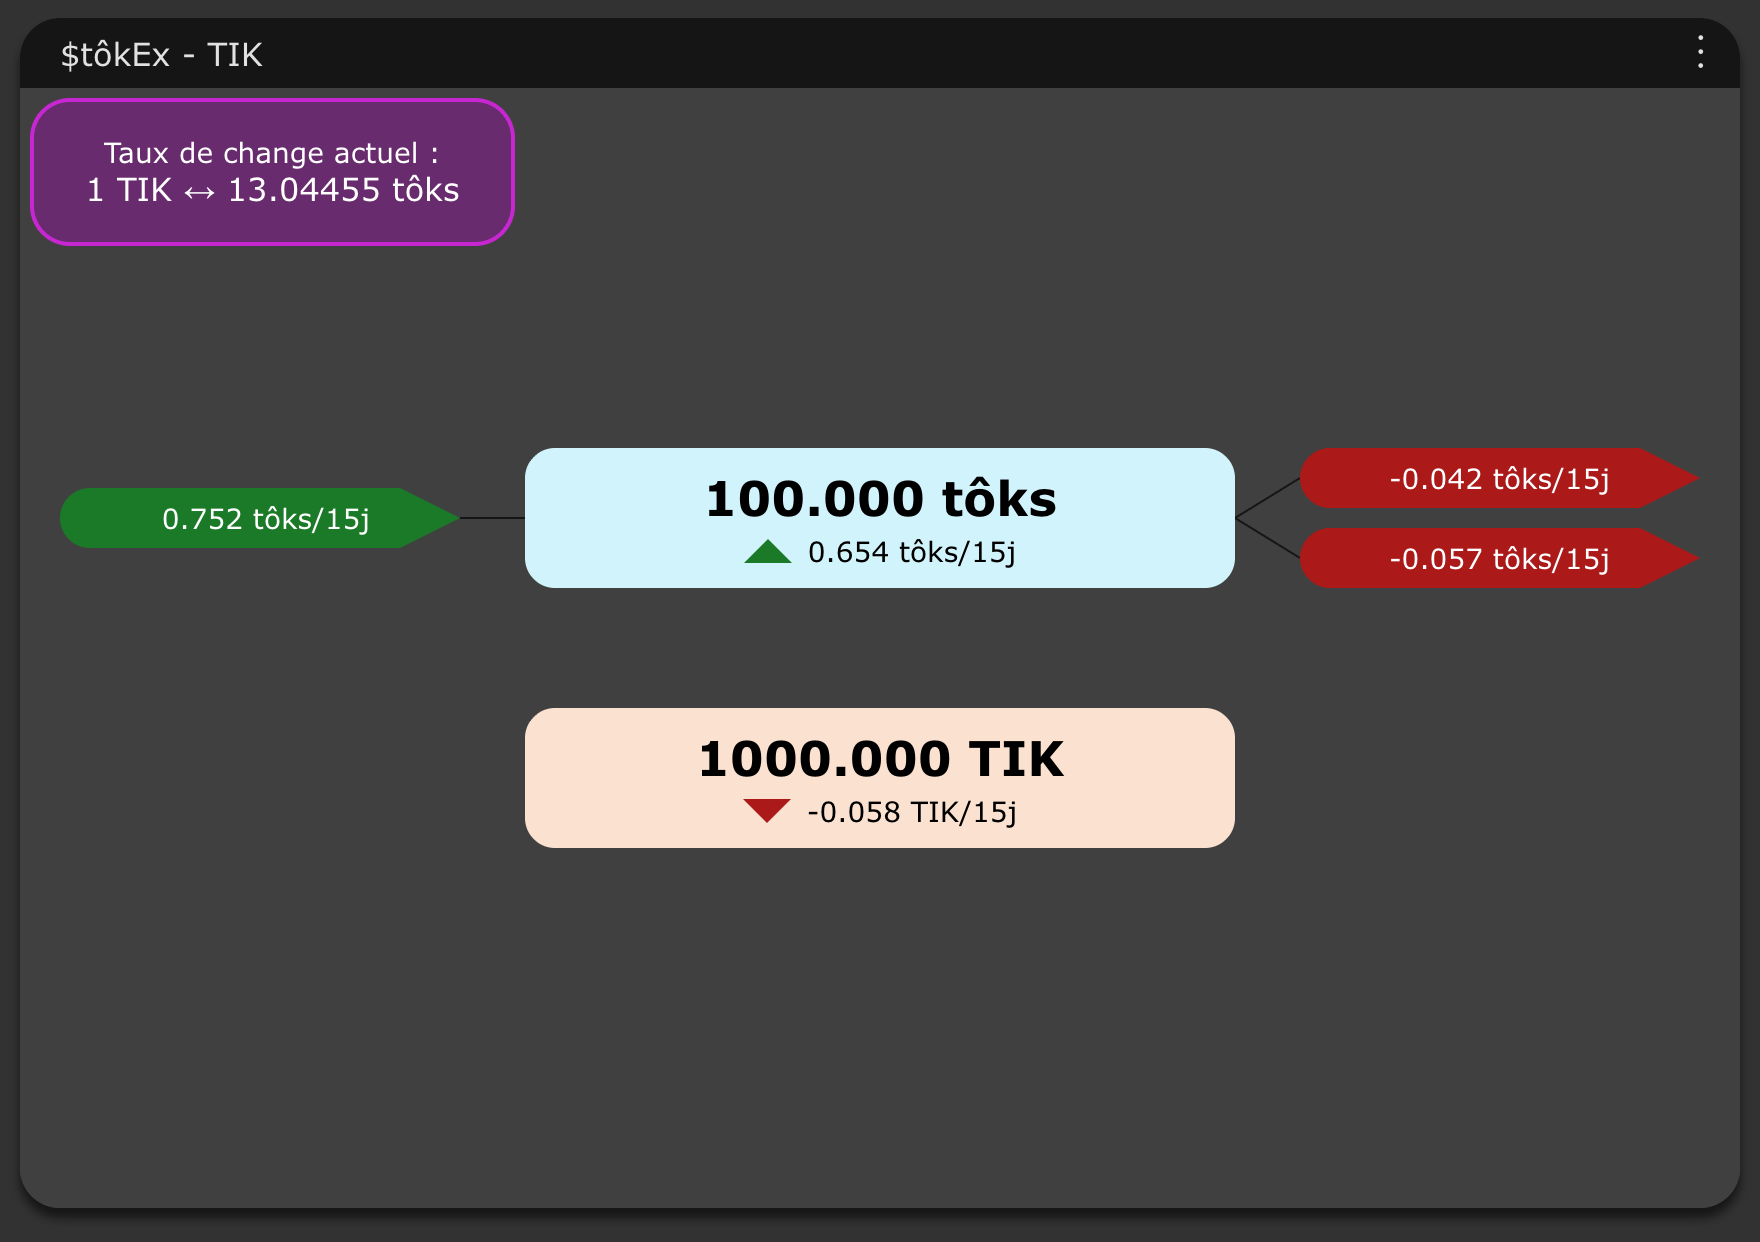
\includegraphics[width=0.75\textwidth]{reference_implementation_ui_1.png}\\[8pt]
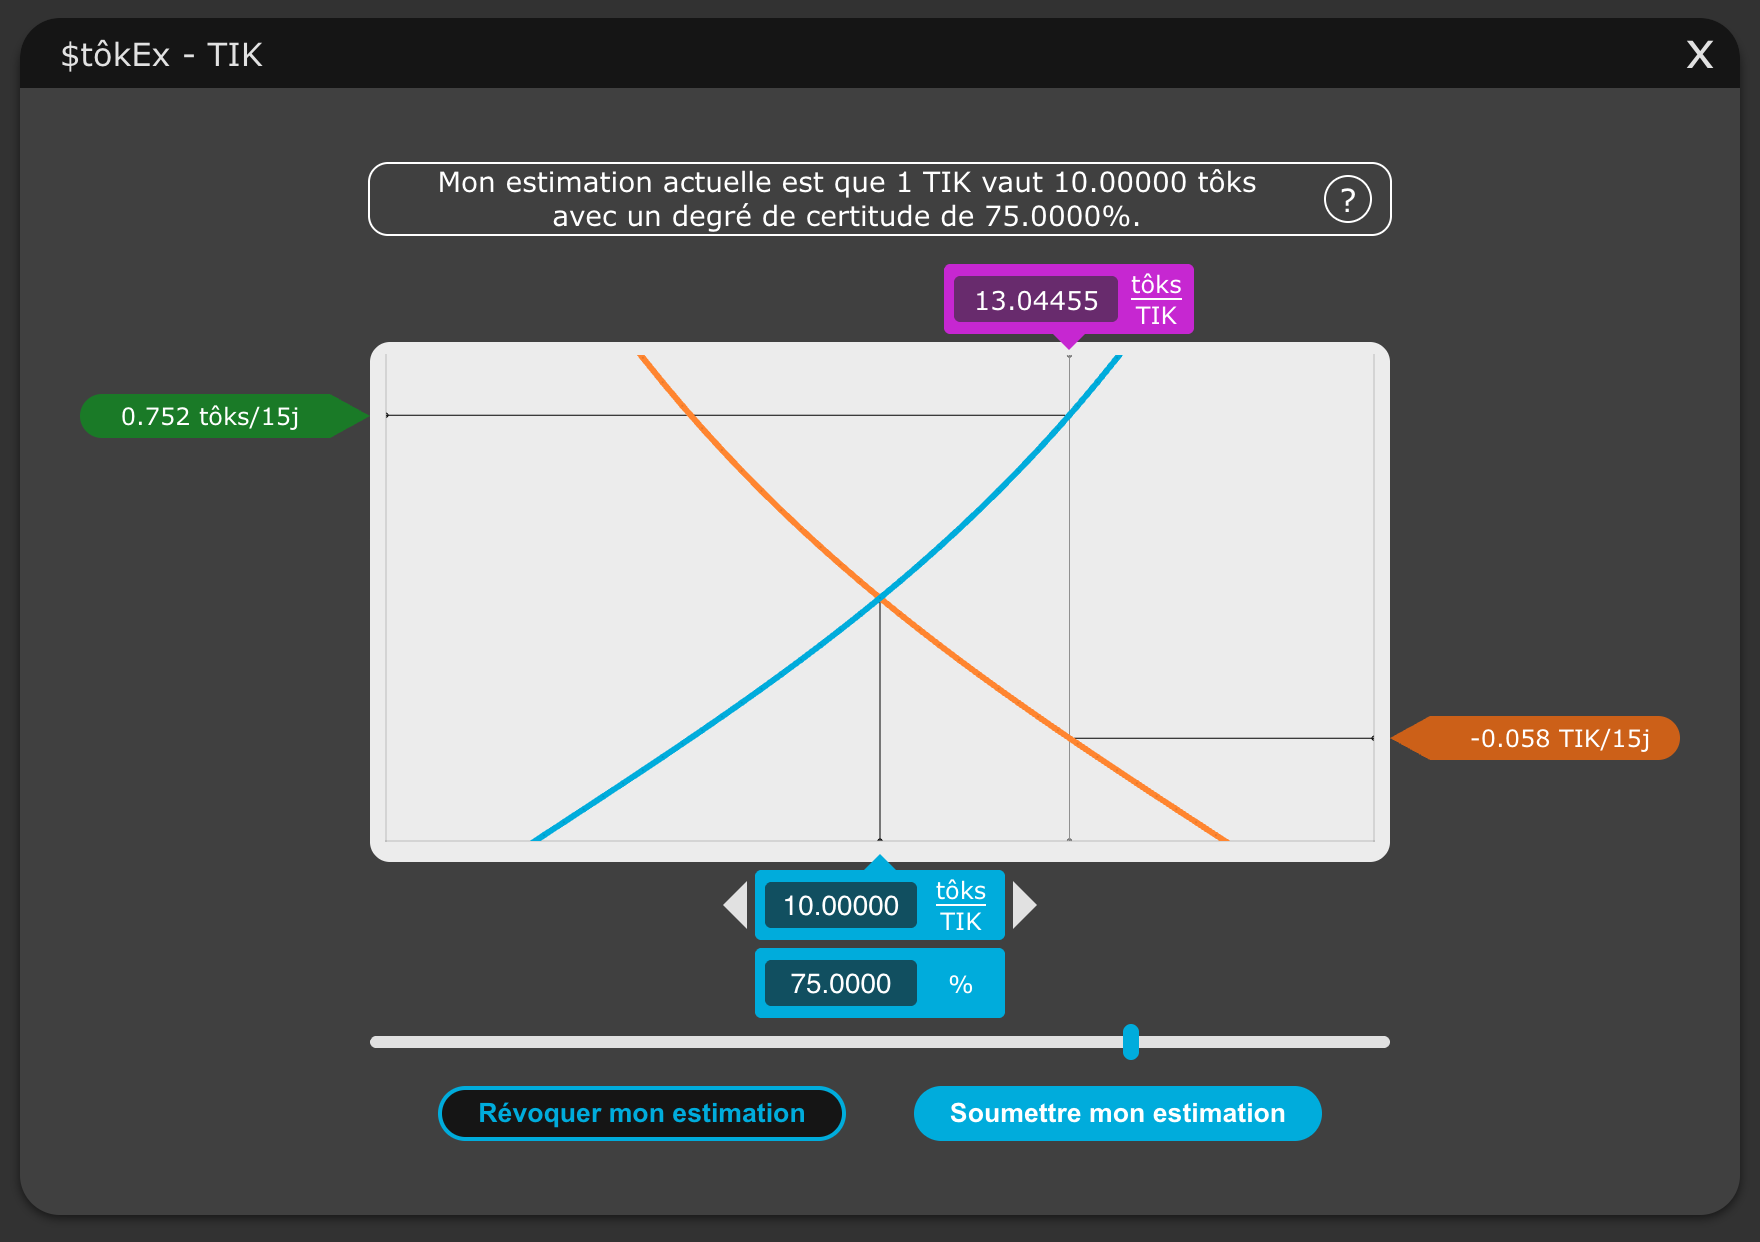
\includegraphics[width=0.75\textwidth]{reference_implementation_ui_2.png}
\caption{The reference implementation of the \StokEx{} in the \tok{} system, shown against a fictional foreign currency, the TIK. \emph{Top:} the market view --- the current exchange rate, each account's balance (here $100$~\tok{}s and $1000$~TIK), and the two exchange velocities, quoted per $15$~days (the universal-income velocity is 1~\tok{} per $15$~days). \emph{Bottom:} the same participant declaring their two inputs, an estimate ($1$~TIK${}={}10$~\tok{}s) and a degree of confidence ($75\%$), with the response curves the mechanism derives from them.}
\label{figRefImplUI}
\end{figure}

Each participant holds a dedicated pair of market accounts (one per asset) with the same owner, and solvency is handled by per-asset tolerance thresholds. Market sums are computed with compensated (Kahan~\cite{Kahan1965}) summation in extended precision, updates are incremental, in $O(N \log N)$ overall (the solvency checklist is processed in sorted order of the estimates, the participant farthest from the market price always lying at one of its two ends), and the trader function is evaluated in the shifted form \eqref{eqShiftedForm}.

The \tok{} is also the one relaxation of the regular-asset assumption: it carries a continuous disintegration at rate $k$, acting on the balances independently of the exchange velocities (consistently with principle 1, \emph{equilibrium and conservation}: the \StokEx{} itself only transfers). Between two events, \tok{} balances obey $dn_i/dt = \dot{X}_i - k\, n_i$; the balance updates of the outer algorithm use the closed-form exponential solution, and the emptying time of a \tok{} account becomes $\frac{1}{k} \ln\left(1 - k\, n_i / \dot{X}_i\right)$, a strictly increasing function of \eqref{eqDeltaT}.

Since $k$ is the same for every \tok{} account (a single disintegration rate applies to the whole \tok{} asset), this transform is monotonic within that homogeneous group, and \eqref{eqDeltaT} can therefore be minimized before it is applied: the implementation tracks the linear \eqref{eqDeltaT} for every account, takes the minimum \emph{separately} among the \tok{}-selling accounts and among the accounts selling the foreign currency (which carries no disintegration and needs no transform), applies the logarithm once, to the former minimum only, in the numerically stable $\operatorname{log1p}$ form, and compares the two resulting candidates. The event-driven structure of the two algorithms is unchanged and the stepping remains exact.

\clearpage

% ----------------------------------------------------------------------
\section{Market analysis}
% ----------------------------------------------------------------------

In this section we build some additional mathematical tools that may provide helpful insights into a market that uses the \StokEx{} algorithm. Chief among these is the fact that, from the point of view of any outside participant, the whole market behaves exactly like a single participant. This gives an intuitive picture of the market and underlies several of the tools developed below. Among other things, these tools can help a participant choose a good estimate and degree of confidence from a single, well-informed look at the market, rather than continuous monitoring --- directly serving the \emph{accessibility} goal set out earlier.

\subsection{Market behavior}\label{secMarketBehavior}
% ----------------------------------------------------------------------

We define the market behavior as the sum of the behavior of all its participants \eqref{eqExchangeVelocities}, evaluated at a common probe price in place of the market price. This gives
\begin{align}
    \dot{X}_\Omega^\alpha &= \sum_i w_i \left( \left( \frac{\priceAB_z}{\priceAB_i}\right)^2 - \frac{\priceAB_i}{\priceAB_z} \right) \dot{R} \,, \nonumber\\
    \dot{X}_\Omega^\beta  &= \sum_i w_i \left( \left( \frac{\priceBA_z}{\priceBA_i}\right)^2 - \frac{\priceBA_i}{\priceBA_z} \right) \dot{R} \priceBA_i \,, \label{eqDefMarketBehavior}
\end{align}
where $\priceAB_z$ is the probe price: an arbitrary strictly positive price, distinct in general from the market price $\priceAB_\Omega$, at which we choose to evaluate the aggregate response of the market. If $\priceAB_z = \priceAB_\Omega$ then the market is in equilibrium (by definition of $\priceAB_\Omega$) and $\dot{X}_\Omega^\alpha=\dot{X}_\Omega^\beta=0$. However, if a new participant were added to the market, we know that the market price would change. The market behavior allows us to know how the ``old'' market will react, or in other words at what velocity it will exchange with the new participant. Indeed, given the new participant's inputs, we can calculate the new market price using~\eqref{eqMarketPrice}, which gives us $\priceAB_z$ that allows us to calculate the market behavior we just defined.

\subsection{Total market weight}
% ----------------------------------------------------------------------

\textbf{Claim.} The whole market can be thought of as a single participant: from the point of view of a new participant entering the market, it is not possible to distinguish if the exchange is taking place with a diverse collection of participants with various estimates $(\priceAB_i,\, \theta_i)$ or a single participant with an aggregate estimate $\priceAB_\Omega$ (the market price itself) and an aggregate degree of confidence $\Theta_\Omega$, defined below.

We prove this claim in Annex~\ref{secProofTotalMarketWeight}, by showing that there exists a total market weight $W_\Omega$ such that the market behavior defined in \eqref{eqDefMarketBehavior} can be written in the same closed form as a single participant's exchange velocities \eqref{eqExchangeVelocities}, with $i \to \Omega$:
\begin{align}
    \dot{X}_\Omega^\alpha &= W_\Omega \left(\left(\frac{\priceAB_z}{\priceAB_\Omega}\right)^2-\frac{\priceAB_\Omega}{\priceAB_z}\right) \dot{R} \,, \nonumber\\
    \dot{X}_\Omega^\beta &= W_\Omega \left(\left(\frac{\priceBA_z}{\priceBA_\Omega}\right)^2-\frac{\priceBA_\Omega}{\priceBA_z}\right) \dot{R} \priceBA_\Omega \,, \label{eqMarketBehavior}
\end{align}
where the total market weight is given by
\begin{equation}
   W_\Omega = \priceBA_\Omega \sum_i w_i \priceAB_i\,. \label{eqTotalMarketWeight}
\end{equation}
Using the expression \eqref{eqMarketPrice} for the market price, we can also write the total market weight in a second form that may be useful in certain situations
\begin{equation}
   W_\Omega = \priceAB_\Omega^2 \sum_i w_i \priceBA_i^2\,. \label{eqTotalMarketWeight2}
\end{equation}

Consequently, we can define the total market degree of confidence (using the inverse of the  weighting factor function \eqref{eqFunctionW}) as
\begin{equation}
   \Theta_\Omega = \frac{200\%}{\pi} \arctan \left( 3 \, W_\Omega\right) \,. \label{eqTotalMarketDegree}
\end{equation}

An important takeaway from this analysis is that the total market weight $W_\Omega$ can serve as a useful index that indicates the ``stiffness'' of the market. A market with a large $W_\Omega$ will resist more strongly to a change in market price $\priceAB_\Omega$. Moreover, we can see from \eqref{eqTotalMarketWeight} that the market weight increases with each new participant to the market (unless, of course, the old participants decide to change their estimate). This suggests that a market with a large number of participants using the \StokEx{} algorithm would have a relatively stable market price.

\subsection{Average participant estimate}
% ----------------------------------------------------------------------

From the total market weight, we can simply derive the average participant weight as
\begin{equation}
    w_\Omega = \frac{W_\Omega}{N_\Omega} \,, \label{eqAverageParticipantWeight}
\end{equation}
where $N_\Omega$ is the number of participants included in the market, and the average participant degree of confidence as
\begin{equation}
    \theta_\Omega = \frac{200\%}{\pi} \arctan \left( 3 \, w_\Omega\right) \,. \label{eqAvergageParticipantDegree}
\end{equation}

This result, combined with the fact that we can aggregate a group of participants and treat it as a single participant using \eqref{eqMarketBehavior}, can be very useful if we want to compare the average behavior of different sub groups of participants (assuming that we have extra data about them). For instance, in the case of an international market we would be able to tell how the average participant of a certain country perceives the value of an asset compared to the average participant of another country.


\subsection{Market update}\label{secMarketUpdate}
% ----------------------------------------------------------------------

Let's say we have a market $\Omega$ with a certain participant $j$ whose initial estimate is $(\priceAB_{j_1},\, \theta_{j_1})$. Given that estimate, and that of the other participants, we can evaluate the initial market price $\priceAB_{\Omega_1}$ using \eqref{eqMarketPrice} and the initial total market weight $W_{\Omega_1}$ using \eqref{eqTotalMarketWeight}.

If participant $j$ changes their estimate to $(\priceAB_{j_2},\, \theta_{j_2})$, then the new market price will be
\begin{equation}
    \priceAB_{\Omega_2} = \left( \frac{W_{\Omega_1}\priceAB_{\Omega_1} - w_{j_1} \priceAB_{j_1} + w_{j_2} \priceAB_{j_2}}{W_{\Omega_1} \priceBA_{\Omega_1}^2 - w_{j_1}\priceBA_{j_1}^2 + w_{j_2}\priceBA_{j_2}^2}\right)^{1/3} \, ,
\end{equation}
and the new total market weight will be
\begin{equation}
    W_{\Omega_2} = \priceBA_{\Omega_2} \left( W_{\Omega_1}\priceAB_{\Omega_1} - w_{j_1} \priceAB_{j_1} + w_{j_2} \priceAB_{j_2} \right) \, .
\end{equation}

\subsection{Analogous variance of the participants' estimate}
% ----------------------------------------------------------------------

By rewriting \eqref{eqTotalMarketWeight} as
\begin{equation}
    \priceAB_\Omega = \sum_i \frac{w_i}{W_\Omega} \priceAB_i\,,
\end{equation}
we get an expression that makes the market price appear as a weighted average in a statistical sense.

Following this analogy, we derive in Annex~\ref{secStatisticalInterpretation} a quantity that we call the analogous variance of the participants' estimate, which we define as
\begin{equation}
    \sigma_{\priceAB}^2 = \frac{1}{W_\Omega} \sum_i w_i \priceAB_i^2 - \priceAB_\Omega^2\,.
\end{equation}
By taking the square root, we get the analogous standard deviation of the participants' estimate
\begin{equation}
    \sigma_{\priceAB} = \sqrt{\frac{1}{W_\Omega} \sum_i w_i \priceAB_i^2 - \priceAB_\Omega^2}\,.
\end{equation}

In order to derive this result, we had to imply that, in some sense, $w_i/W_\Omega$ corresponds to the probability that a participant estimates the price of $\priceAB$ at $\priceAB_i$ in a context where each participant has the same weight. Since this is not actually the case in the context of the \StokEx{}, we must be careful with the use of the analogous variance and the analogous standard deviation. Nonetheless, these quantities still offer useful insight into the distribution of the participants' estimates, weighted toward the more confident ones.

% ----------------------------------------------------------------------
\section{Conclusion}
% ----------------------------------------------------------------------

Starting from two sets of assumptions --- four \emph{fair-market} principles (\emph{equilibrium and conservation}, \emph{exchange at market price}, \emph{no bias between participants}, and \emph{no bias between assets}) and four \emph{rational-trader} principles (\emph{buy low}, \emph{sell high}, \emph{urgency grows with the gap}, and \emph{urgency grows with confidence}) --- we were led to a mathematical framework for the continuous exchange of two fungible assets.
Although each principle is, on its own, intuitive and hard to object to, the mathematical framework they jointly force is remarkably constrained: a simple one-parameter family of trader functions (from which we picked the member $p = 2$, giving $f(x) = x^2 - 1/x$), a symmetric pair of exchange velocities, and a market price in closed form (Eq.~\eqref{eqMarketPrice}) that is unique and clears both assets at every instant.

In a sense, the \StokEx{} is an idealized market: supply and demand clear exactly and continuously, at a single price given in closed form, the Walrasian ideal made computable rather than approached by iteration. That so tightly constrained a framework is even consistent is surprising in itself. More striking still, it is self-similar: the aggregate of many participants behaves exactly as one participant (Annex~\ref{secProofTotalMarketWeight}), a property never assumed but forced by the assumptions, which invites deeper thoughts about the numerical modeling of markets in general.

The full range of applications of the \StokEx{} remains open. Its continuous clearing seems a natural fit for goods produced and consumed as a flow rather than in discrete lots (electricity being the obvious example, where supply and demand must balance in real time). It may also serve as a lightweight layer of rational agents in large-scale economic simulations: each participant is summarized by two numbers, its response is a handful of floating-point operations on the trader function, and an entire market of $N$ participants clears in $O(N \log N)$ while aggregating exactly into a single representative participant, so markets can be nested and composed cheaply.

Beyond any particular application, the insight we would most like to highlight concerns the reference exchange velocity $\dot{R}$ by which every participant's trading is scaled. Giving it a meaning requires a unit of value that is stable in time, a yardstick against which estimates of relative value can be made. Such a stable unit is, in essence, an ideal currency: one whose value does not drift, $d\dot{R}/dt = 0$. In fact, the existence of such a currency is the basis for the \tok{} system developed by Smoothop (a non-profit organization dedicated to the socioecological transition), in which $\dot{R}$ is the universal-income velocity of 1~\tok{}per 15~days.

Every central result of this document --- the closed-form market price and its uniqueness, the exchange taking place exactly at that price, and the exact aggregation of the whole market into a single participant (Annex~\ref{secProofTotalMarketWeight}) --- is machine-checked in Lean~4 / mathlib. The \StokEx{}, together with the entire admissible family of trader functions (Annex~\ref{secTraderFamily}), is disclosed here as prior art.

\clearpage
% ----------------------------------------------------------------------
\section{Annexes: Mathematical Proofs}
% ----------------------------------------------------------------------

\placeholder{\textbf{[To be completed before submitting]}~ Insert here fixed url tag \texttt{stokex-defpub-2026-08} :
\url{https://github.com/smoothop-org/tok-system/tree/stokex-defpub-2026-08/publications/stokex/}}

\subsection{The reference exchange velocity}\label{secReferenceVelocityBias}
% ----------------------------------------------------------------------

The reference velocity $\dot{R}$ in \eqref{eqExchangeSymmetry} is defined in terms of asset A, which seems to break principle 4 (\emph{no bias between assets}).
In a weak sense this is true, but it's a matter of user interface design rather than a mathematical breaking of symmetry.

\textbf{A per-participant reference exchange velocity is a weight.} Nothing forces $\dot{R}$ to be common.
Let each participant $i$ declare their own reference exchange velocity in either asset $\dot{R}_i^\alpha$ or $\dot{R}_i^\beta$ so that not a trace of bias between assets remains.
Then we can rewrite \eqref{eqExchangeSymmetry} as
\begin{align*}
\dot{X}^\alpha_i &= w\!\left(\theta_i\right)\, f\!\left(\frac{\hspace{2pt}\priceAB_\Omega}{\priceAB_i} \right) \, \dot{R}_i^\alpha \, , \\
\dot{X}^\beta_i &=  w\!\left(\theta_i\right)\, f\!\left(\frac{\hspace{2pt}\priceBA_\Omega}{\priceBA_i} \right) \, \dot{R}_i^\beta \,,
\end{align*}
with the identity
\begin{align*}
    \dot{R}_i^\alpha &= \dot{R}_i^\beta \priceAB_i \, , \\
    \dot{R}_i^\beta &= \dot{R}_i^\alpha \priceBA_i \,.
\end{align*}
This expression is unchanged under an $\alpha \leftrightarrow \beta$ swap, so principle 4 (\emph{no bias between assets}) holds.

Now the important observation is that $\dot{R}_i$ never appears alone; it is always multiplied by $w\!\left(\theta_i\right)$, so only one parameter is needed.
Indeed, we can absorb $\dot{R}_i$ in the participant's weight $\dot{w}_i := w\!\left(\theta_i\right)\dot{R}_i$ and derive all the document's results as before.
The point is that we need one parameter from each participant to scale their trader-function output according to their degree of confidence or willingness to trade.

\textbf{What a common reference exchange velocity buys} is a way to compare different participants' degrees of confidence on a $[0,100)\%$ domain.
Also, in the reference implementation of the \tok{} system (Sec.~\ref{secReferenceImplementation}), the universal income
rate appears as a natural choice of reference velocity.

\textbf{Disclosure.} An exchange mechanism scaling each participant's exchange velocities
by an individual reference velocity, in either asset, however declared or derived, is
anticipated by this document.


\subsection{The family of admissible trader functions}\label{secTraderFamily}
% ----------------------------------------------------------------------

The \StokEx{} defines its trader function as $f(x) = x^2 - 1/x$. This annex makes precise which part of that choice is forced by the principles and which part is a design decision, and it discloses the whole family of admissible alternatives.

\textbf{What the principles force.} Let $f$ be any candidate trader function, used symmetrically by both assets as in \eqref{eqExchangeSymmetry}, and write $x_i = \priceAB_\Omega / \priceAB_i$. The two exchange velocities of participant $i$ are then $\dot{X}^\alpha_i = w_i f(x_i)\, \dot{R}$ and $\dot{X}^\beta_i = w_i f(1/x_i)\, \dot{R} \priceBA_i$. Principle 2 (\emph{exchange at market price}) requires $-\dot{X}^\alpha_i / \dot{X}^\beta_i = \priceAB_\Omega = x_i \priceAB_i$ for every market state, which simplifies to $f(1/x_i) = -f(x_i)/x_i$. Since $x_i$ ranges over all of $(0,\infty)$ as the market state varies, $f$ must satisfy the functional equation
\begin{equation}
    f(1/x) = -\frac{f(x)}{x} \qquad \text{for all } x > 0\,. \label{eqFunctionalEquation}
\end{equation}
At $x = 1$, \eqref{eqFunctionalEquation} gives $f(1) = -f(1)$, hence $f(1) = 0$: not trading at one's own estimate is not an extra hypothesis, it is a consequence of exchanging two symmetric assets at a single market price. The equation also determines $f$ on $(0,1)$ from its values on $(1,\infty)$: the selling behavior is the reflection of the buying behavior. Concretely, in absolute value, a participant facing a market at twice their estimate behaves exactly as one facing half of it, with the roles of the two assets exchanged (each velocity counted in the reference unit of its own asset); this mirror symmetry is shared by every admissible trader function, and is the one visible in Fig.~\ref{figExchangeSymmetry}.

\textbf{The closed-form family.} Consider the power pairs
\begin{equation}
    f_p(x) = x^p - x^q\,, \qquad q = 1 - p\,, \quad p \geq 1\,. \label{eqTraderFamily}
\end{equation}
Every member satisfies \eqref{eqFunctionalEquation}, since $q - 1 = -p$ and $p - 1 = -q$. For $p \geq 1$ the member is strictly increasing on $(0, \infty)$, with $f_p'(x) = p\,x^{p-1} + (p-1)\,x^{-p} > 0$, and therefore satisfies principles 5 to 7 (\emph{buy low} through \emph{urgency grows with the gap}; for $1/2 < p < 1$ monotonicity fails near $0$, and $p = 1/2$ gives the zero function). Replacing $f$ by $f_p$ in \eqref{eqExchangeSymmetry} and solving the equilibrium condition \eqref{eqEquilibrium} yields the market price in closed form,
\begin{equation}
    \priceAB_\Omega = \left( \frac{\displaystyle \sum_i w_i \priceAB_i^{\,p-1}}{\displaystyle \sum_i w_i \priceBA_i^{\,p}} \right)^{1/(2p-1)}\,, \label{eqFamilyPrice}
\end{equation}
and the slope at the equilibrium point is $f_p'(1) = 2p - 1$, so that the degree-of-confidence map of the member reads $w = \frac{1}{2p-1} \tan\left(\pi\,\theta/200\,\%\right)$. All the results of this document (uniqueness of the price, aggregation of the market into a single participant, the two algorithms) carry over member by member. More generally, any combination $\sum_p c_p f_p$ with nonnegative coefficients satisfies \eqref{eqFunctionalEquation} and the principles, though the closed form \eqref{eqFamilyPrice} is then lost.

\textbf{What singles out $p = 2$.} The first member, $f_1(x) = x - 1$, has a bounded selling side: $f_1(x) > -1$ for all $x > 0$, so a participant's urgency would saturate at $w_i \dot{R}$ no matter how far the market price drops below their estimate. For every $p > 1$, both sides are unbounded: $f_p \to +\infty$ as $x \to \infty$ and $f_p \to -\infty$ as $x \to 0^+$. A second consideration is computational, and it stems from the accessibility goal: a market that charges no fees must keep the evaluation of its trader function as cheap as possible, which favors integer exponents (Laurent polynomials) --- needing only multiplications and a single reciprocal --- over fractional powers, whose transcendental $\exp/\log$ evaluation costs far more at every step. Among the members with integer exponents, the smallest one with unbounded urgency on both sides is therefore $p = 2$:
\begin{equation*}
    f_2(x) = x^2 - \frac{1}{x}\,,
\end{equation*}
the trader function \eqref{eqTraderFunction} of the \StokEx{}, whose slope $2p - 1 = 3$ is the factor of \eqref{eqFunctionW}.

\textbf{Disclosure.} The whole family \eqref{eqTraderFamily}, together with the corresponding market price \eqref{eqFamilyPrice} and degree-of-confidence map, is part of the present disclosure: an exchange mechanism obtained by substituting any member $f_p$ (or any nonnegative combination of members) for the trader function of the \StokEx{} is anticipated by this document.

\subsection{The family of admissible weight functions}\label{secWeightFamily}
% ----------------------------------------------------------------------

The \StokEx{} maps a participant's degree of confidence onto their weight through the tangent function \eqref{eqFunctionW}.
This annex makes precise which part of that choice is forced by the principles and which part is a user interface design decision.

\textbf{What the principles force.} Principle 8 (\emph{urgency grows with confidence}) requires only that $w: [0,100\%) \to [0,+\infty)$ be strictly increasing, with $w(0) = 0$ (no conviction, no trade).
Nothing else about $w$ enters principles 1--8: every other result in this document is derived using the participants' weights $w_i$ alone, and never from the functional form that produced $w_i$ from $\theta_i$.

\textbf{What singles out the tangent map.} The particular choice \eqref{eqFunctionW} is what makes $\theta_i$ coincide with a geometrical angle, the equilibrium slope of the participant's own response curve (Annex~\ref{secProofDegree}); this interpretation, and the discretization used in the reference implementation (Sec.~\ref{secReferenceImplementation}), are properties of that particular member, not requirements of the algorithm.

\textbf{Disclosure.} The whole family of strictly increasing functions $w$ with $w(0) = 0$, substituted for \eqref{eqFunctionW} in an otherwise unchanged \StokEx{}, is part of the present disclosure: an exchange mechanism that scales participants' exchange velocities by any such weight --- however that weight is computed from a declared degree of confidence or equivalent conviction signal --- is anticipated by this document.


\subsection{Proof that the participant's degree of confidence corresponds to a geometrical angle}\label{secProofDegree}
% ----------------------------------------------------------------------

In Fig.~\ref{figDegree} we plot a participant's exchange velocity for asset A \eqref{eqExchangeVelocities} on a 2-D graph with normalized axes, such that
\begin{equation*}
    x = \frac{\hspace{2pt}\priceAB_\Omega}{\priceAB_i}\,\text{ and }\,
    y = \frac{\dot{X}_i^\alpha}{\dot{R}} \,.
\end{equation*}
Given our normalized quantities $x$ and $y$, the expression for the exchange velocity becomes
\begin{equation*}
    y = w \left(x^2 - \frac{1}{x}\right)
\end{equation*}

In Fig.~\ref{figDegree}, we define $\theta$ as being the angle between the horizontal axis $y=0$ and the slope of the exchange at the point where they cross. Geometrically, this corresponds to
\begin{equation*}
    \tan \left( \theta \right) = \left.\frac{dy}{dx}\right|_{y=0} = 3\, w
\end{equation*}
Thus, the relation between $\theta$ and $w$ is
\begin{equation*}
    w = \frac{1}{3}\tan \left(\theta\right)\,.
\end{equation*}

The same argument holds true if we want to plot a participant's exchange velocity using a logarithmic scale in $x$ (see Fig.~\ref{figDegreeLog}). In that case, the normalized axes are
\begin{equation*}
    x = \ln\!\left(\frac{\hspace{2pt}\priceAB_\Omega}{\priceAB_i}\right) \,\text{ and }\,
    y = \frac{\dot{X}_i^\alpha}{\dot{R}}\,,
\end{equation*}
and the expression for the exchange velocity becomes
\begin{equation*}
    y = w \left(\exp(2x) - \exp(-x)\right) \, .
\end{equation*}
Again, we find that
\begin{equation*}
    \tan \left( \theta \right) = \left.\frac{dy}{dx}\right|_{y=0} = 3\, w \,,
\end{equation*}
which leads to the relation between $\theta$ and $w$ that we were looking for
\begin{equation*}
    w = \frac{1}{3}\tan \left(\theta\right)\,.
\end{equation*}

Let us note that the last expression assumes that the angle $\theta$ is in radians and contained between 0 and $\pi/2$. To get the expression \eqref{eqFunctionW}, we linearly map $[0,\pi/2)$ to $[0,100)\%$. This leads to
\begin{equation*}
    w = \frac{1}{3}\tan \left(\frac{\pi\, \theta}{200\%}\right)\,,
\end{equation*}
in which $\theta$ is the participant's ``degree of confidence'' contained between 0\% and 100\%.

\subsection{Proof that the exchange-velocity function implies an exchange at market price}\label{secProofExchangeAtMarketPrice}
% ----------------------------------------------------------------------

We want to show that the expressions for a participant's exchange velocities defined in \eqref{eqExchangeVelocities} automatically satisfy the principle \eqref{eqExchangeAtMarketPrice}.

By constructing the right side of \eqref{eqExchangeAtMarketPrice}, using the expressions in \eqref{eqExchangeVelocities}, we get
\begin{align*}
    -\frac{\dot{X}^\alpha_i}{\dot{X}^\beta_i} &= -\frac{\hspace{-29pt}w_i \left( \left( \frac{\hspace{2pt}\priceAB_\Omega}{\priceAB_i}\right)^2 - \frac{\priceAB_i}{\hspace{2pt}\priceAB_\Omega} \right) \dot{R}}{w_i \left( \left( \frac{\hspace{2pt}\priceBA_\Omega}{\priceBA_i}\right)^2 - \frac{\priceBA_i}{\hspace{2pt}\priceBA_\Omega} \right) \dot{R} \priceBA_i}\\
    &= \frac{\hspace{12pt}\frac{\priceAB_i}{\hspace{2pt}\priceAB_\Omega} - \left( \frac{\hspace{2pt}\priceAB_\Omega}{\priceAB_i}\right)^2 }{\left( \frac{\hspace{2pt}\priceBA_\Omega}{\priceBA_i}\right)^2 - \frac{\priceBA_i}{\hspace{2pt}\priceBA_\Omega}} \priceAB_i\\
    &=\frac{\frac{\priceAB_i^3-\priceAB_\Omega^3}{\priceAB_\Omega \priceAB_i^2}}{\frac{\priceBA_\Omega^3-\priceBA_i^3}{\priceBA_i^2 \priceBA_\Omega}} \priceAB_i\\
    &= \left(\frac{\priceAB_i^3-\priceAB_\Omega^3}{\priceBA_\Omega^3-\priceBA_i^3} \right)\left(\frac{\priceBA_i^2 \priceBA_\Omega}{\priceAB_\Omega \priceAB_i^2} \right)\priceAB_i\\
    &= \left(\frac{\priceAB_i^3-\priceAB_\Omega^3}{\priceBA_\Omega^3-\priceBA_i^3} \right) \left(\priceBA_i^3 \priceBA_\Omega^3\right)\priceAB_\Omega\\
    &= \left( \frac{\priceBA_\Omega^3 - \priceBA_i^3}{\priceBA_\Omega^3 - \priceBA_i^3}\right) \priceAB_\Omega \\
    &= \priceAB_\Omega \,.
\end{align*}
\begin{flushright}
Q.E.D.
\end{flushright}

\subsection{Proof that the expression for the market price corresponds to the equilibrium between supply and demand}\label{secProofMarketprice}
% ----------------------------------------------------------------------

By making the hypothesis that~\eqref{eqEquilibrium} holds for asset A and by applying principle number 2 (\emph{exchange at market price}), stating that the market price is the same for every participant at any given time and that the market price is strictly positive, we can derive expression \eqref{eqMarketPrice} as such:
\begin{align*}
    0 &= \sum_i \dot{X}_i^\alpha\\
    0 &= \sum_i w_i \left( \left( \frac{\hspace{2pt}\priceAB_\Omega}{\priceAB_i}\right)^2 - \frac{\priceAB_i}{\hspace{2pt}\priceAB_\Omega} \right) \dot{R} \\
    0 &= \sum_i w_i \left( \priceBA_i^2 - \priceBA_\Omega^3 \priceAB_i \right) \priceAB_\Omega^2 \dot{R}\\
    0 &= \sum_i w_i \priceBA_i^2 - \priceBA_\Omega^3 \sum_i w_i \priceAB_i\\
    \priceAB_\Omega &= \left( \frac{\displaystyle \sum_i w_i \priceAB_i}{\displaystyle \sum_i w_i \priceBA_i^2}\right)^{1/3} \,.
\end{align*}
\begin{flushright}
Q.E.D.
\end{flushright}
Since we have already proven that
\begin{equation*}
    \sum_i \dot{X}_i^\alpha = 0 \text{ and that }\priceAB_\Omega = -\frac{\dot{X}_i^\alpha}{\dot{X}_i^\beta}\,,
\end{equation*}
we can quickly show that the exchanges of asset~B also satisfy \eqref{eqEquilibrium} in the following manner
\begin{align*}
    \sum_i \dot{X}_i^\beta &= -\priceBA_\Omega \sum_i \dot{X}_i^\alpha\\
    \sum_i \dot{X}_i^\beta &= 0 \,.
\end{align*}
\begin{flushright}
Q.E.D.
\end{flushright}

\subsection{Proof that the market price is unique}\label{secProofUniqueness}
% ----------------------------------------------------------------------

Annex~\ref{secProofMarketprice} is conditional: it shows that \emph{if} an equilibrium price exists, it must be \eqref{eqMarketPrice}. This annex closes the argument by showing that exactly one equilibrium price always exists, so that the market price of principle 1 (\emph{equilibrium and conservation}) is well defined and the inner algorithm is deterministic.

\textbf{Conditions.} Every estimate is strictly positive, every weight is nonnegative, and at least one trading participant carries a strictly positive weight:
\begin{equation*}
    \priceAB_i > 0 \ \text{ for all } i\,, \qquad w_i \geq 0 \ \text{ for all } i\,, \qquad \exists\, j: w_j > 0\,.
\end{equation*}

\textbf{Claim.} Under these conditions, there is exactly one strictly positive price at which the market is in equilibrium, and it is the one given by \eqref{eqMarketPrice}.

\textbf{Proof.} Consider the market behavior $\dot{X}_\Omega^\alpha$ of \eqref{eqDefMarketBehavior} as a function of the probe price $\priceAB_z > 0$:
\begin{equation*}
    \dot{X}_\Omega^\alpha(\priceAB_z) = \sum_i w_i \left( \left(\frac{\priceAB_z}{\priceAB_i}\right)^2 - \frac{\priceAB_i}{\priceAB_z} \right) \dot{R}\,.
\end{equation*}
Each term with $w_i > 0$ is strictly increasing in $\priceAB_z$, since
\begin{equation*}
    \frac{d}{d\priceAB_z}\left[ w_i \left( \left(\frac{\priceAB_z}{\priceAB_i}\right)^2 - \frac{\priceAB_i}{\priceAB_z} \right) \right] = w_i \left( \frac{2\priceAB_z}{\priceAB_i^2} + \frac{\priceAB_i}{\priceAB_z^2} \right) > 0\,,
\end{equation*}
and each term with $w_i = 0$ vanishes identically. As at least one weight is strictly positive, $\dot{X}_\Omega^\alpha$ is strictly increasing on $(0, \infty)$. Moreover, $\dot{X}_\Omega^\alpha(\priceAB_z) \to -\infty$ as $\priceAB_z \to 0^+$ (the $-\priceAB_i/\priceAB_z$ terms dominate) and $\dot{X}_\Omega^\alpha(\priceAB_z) \to +\infty$ as $\priceAB_z \to \infty$ (the quadratic terms dominate). Since $\dot{X}_\Omega^\alpha$ is continuous and strictly increasing with these limits, it vanishes at exactly one $\priceAB_z > 0$. By Annex~\ref{secProofMarketprice}, that zero is \eqref{eqMarketPrice}.
\begin{flushright}
Q.E.D.
\end{flushright}

\textbf{Corollary.} Every term of $\dot{X}_\Omega^\alpha$ is nonpositive at $\priceAB_z = \min_i \priceAB_i$ (all ratios $\priceAB_z/\priceAB_i \leq 1$) and nonnegative at $\priceAB_z = \max_i \priceAB_i$; the equilibrium price therefore always lies between the smallest and the largest estimate of the trading participants.

\subsection{Proof that the total market behaves as a single participant}\label{secProofTotalMarketWeight}
% ----------------------------------------------------------------------

In \eqref{eqDefMarketBehavior}, we defined the market behavior as the sum of the behavior of all its participants
\begin{align*}
    \dot{X}_\Omega^\alpha &= \sum_i w_i \left( \left( \frac{\priceAB_z}{\priceAB_i}\right)^2 - \frac{\priceAB_i}{\priceAB_z} \right) \dot{R} \,,\\
    \dot{X}_\Omega^\beta &= \sum_i w_i \left( \left( \frac{\priceBA_z}{\priceBA_i}\right)^2 - \frac{\priceBA_i}{\priceBA_z} \right) \dot{R} \priceBA_i \,.
\end{align*}
We want to prove that there exists a total market weight $W_\Omega$ such that the market behaves as a single participant, in a way that
\begin{equation*}
    W_\Omega\left(\left(\frac{\priceAB_z}{\priceAB_\Omega}\right)^2-\frac{\priceAB_\Omega}{\priceAB_z}\right) \dot{R} = \sum_i w_i \left( \left( \frac{\priceAB_z}{\priceAB_i}\right)^2 - \frac{\priceAB_i}{\priceAB_z} \right) \dot{R} \,,
\end{equation*}
for any $\priceAB_z$. We treat the asset~A identity first; the asset~B identity then follows as an easy corollary.

Of course, this statement is true in the trivial case when the inputs of each of the $N_\Omega$ participants are $\priceAB_i = \priceAB_\Omega$ and $w_i=W_\Omega / N_\Omega$, but we want to prove that it is in fact true for any participant's inputs.

By looking at the previous expression term by term, we conclude that for it to be true for any $\priceAB_z$, we must satisfy both
\begin{align*}
    W_\Omega \priceBA_\Omega^2 &= \sum_i w_i \priceBA_i^2 \, \text{ and}\\
    W_\Omega \priceAB_\Omega &= \sum_i w_i \priceAB_i\,.
\end{align*}
We can easily satisfy the second expression by setting
\begin{equation*}
    W_\Omega = \priceBA_\Omega \sum_i w_i \priceAB_i\,.
\end{equation*}

Now, we need to verify that this choice also satisfies the first expression
\begin{align*}
    W_\Omega \priceBA_\Omega^2 &= \sum_i w_i \priceBA_i^2 \\
    \left(\priceBA_\Omega \sum_i w_i \priceAB_i\right) \priceBA_\Omega^2 &= \sum_i w_i \priceBA_i^2\\
    \priceBA_\Omega^3 \sum_i w_i \priceAB_i &= \sum_i w_i \priceBA_i^2\\
    \priceAB_\Omega &= \left(\frac{\displaystyle \sum_i w_i \priceAB_i}{\displaystyle \sum_i w_i \priceBA_i^2} \right)^{1/3} \,.
\end{align*}
The last line corresponds to the expression for the market price that we already proved in Annex~\ref{secProofMarketprice}.

\begin{flushright}
Q.E.D.
\end{flushright}

\textbf{Corollary (asset B).} Write $x_i = \priceAB_z/\priceAB_i$ and $x_\Omega = \priceAB_z/\priceAB_\Omega$, and recall the trader function $f(x) = x^2 - 1/x$ \eqref{eqTraderFunction}, so that $\dot{X}_\Omega^\alpha = \sum_i w_i f(x_i) \dot{R} = W_\Omega f(x_\Omega) \dot{R}$ is exactly the identity just proved. Since $\priceBA_z/\priceBA_i = 1/x_i$, the functional equation $f(1/x) = -f(x)/x$ \eqref{eqFunctionalEquation} of Annex~\ref{secTraderFamily} gives $f(\priceBA_z/\priceBA_i) = -f(x_i)/x_i$; moreover $\priceBA_i/x_i = \priceBA_i \priceAB_i/\priceAB_z = 1/\priceAB_z$ for every $i$ (asset~A's estimate and asset~B's estimate of the same participant are reciprocal), the aggregate participant $\Omega$ included. Hence
\begin{align*}
    \dot{X}_\Omega^\beta &= \sum_i w_i\, f\!\left(\priceBA_z/\priceBA_i\right)\, \dot{R}\, \priceBA_i\\
    &= -\dot{R} \sum_i w_i\, f(x_i)\, \frac{\priceBA_i}{x_i}\\
    &= -\frac{\dot{R}}{\priceAB_z} \sum_i w_i\, f(x_i)\\
    &= -\frac{\dot{R}}{\priceAB_z}\, W_\Omega\, f(x_\Omega)\,,
\end{align*}
using the asset~A identity for the last step. Running the same three simplifications backward, with $i$ replaced by $\Omega$, turns the right-hand side back into $W_\Omega f(\priceBA_z/\priceBA_\Omega) \dot{R} \priceBA_\Omega$, which is the asset-B line of \eqref{eqMarketBehavior}.
\begin{flushright}
Q.E.D.
\end{flushright}

\subsection{Behavior of the market as one participant's weight diverges}\label{secProofInfiniteWeight}
% ----------------------------------------------------------------------

We show that the market stays well-behaved when a single participant becomes infinitely confident, $w_\ell \to \infty$ --- equivalently $\theta_\ell \to 100\%$, the supremum of the degree-of-confidence range. Such a participant fixes the market price at their own estimate, yet every exchange velocity remains finite, set entirely by the rest of the market.

\textbf{Reduction to two participants.} Single out participant $\ell$ and aggregate all the others. By Annex~\ref{secProofTotalMarketWeight}, applied to the sub-market of every participant except $\ell$, that rest behaves --- at every probe price --- exactly as one participant with estimate $\priceAB_r$ (its own market price) and weight $W_r$, both finite and independent of $w_\ell$. The full market is then the two-participant system $\{\ell, r\}$, and, the aggregate reproducing the same behavior as the crowd it replaces, its equilibrium price \eqref{eqMarketPrice} is
\begin{equation*}
    \priceAB_\Omega = \left( \frac{w_\ell \priceAB_\ell + W_r \priceAB_r}{w_\ell \priceBA_\ell^2 + W_r \priceBA_r^2} \right)^{1/3} \,.
\end{equation*}

\textbf{The price is pinned to $\ell$'s estimate.} As $w_\ell \to \infty$ the $w_\ell$ terms dominate both numerator and denominator, and since $\priceAB_\ell / \priceBA_\ell^2 = \priceAB_\ell^3$,
\begin{equation*}
    \priceAB_\Omega \longrightarrow \left( \frac{\priceAB_\ell}{\priceBA_\ell^2} \right)^{1/3} = \priceAB_\ell \,.
\end{equation*}
Equivalently, the total market weight \eqref{eqTotalMarketWeight} diverges, $W_\Omega \to \infty$ (hence $\Theta_\Omega \to 100\%$ by \eqref{eqTotalMarketDegree}): the market becomes infinitely stiff and its price no longer responds to the other participants.

\textbf{The velocities stay finite.} At first sight participant $\ell$'s velocity $\dot{X}_\ell^\alpha = w_\ell\, f\!\left(\priceAB_\Omega / \priceAB_\ell\right) \dot{R}$ is the indeterminate product of $w_\ell \to \infty$ and $f\!\left(\priceAB_\Omega / \priceAB_\ell\right) \to f(1) = 0$. Equilibrium resolves it exactly: by \eqref{eqEquilibrium}, for every finite $w_\ell$,
\begin{equation*}
    \dot{X}_\ell^\alpha = -\dot{X}_r^\alpha = -\,W_r\, f\!\left( \frac{\priceAB_\Omega}{\priceAB_r} \right) \dot{R} \,,
\end{equation*}
and the right-hand side depends on $w_\ell$ only through $\priceAB_\Omega$. Letting $w_\ell \to \infty$, with $\priceAB_\Omega \to \priceAB_\ell$ and $W_r, \priceAB_r$ fixed,
\begin{equation*}
    \dot{X}_\ell^\alpha \longrightarrow -\,W_r\, f\!\left( \frac{\priceAB_\ell}{\priceAB_r} \right) \dot{R} \,,
\end{equation*}
a finite limit, and the asset-B velocity follows identically.

It is worth seeing the $\infty \cdot 0$ cancel explicitly, without appealing to equilibrium. The trader function obeys the identity $x\,f(x) = x^3 - 1$, so, writing $x_\ell = \priceAB_\Omega / \priceAB_\ell$,
\begin{equation*}
    \dot{X}_\ell^\alpha = w_\ell\, f(x_\ell)\, \dot{R} = w_\ell\, \frac{x_\ell^3 - 1}{x_\ell}\, \dot{R} \,,
\end{equation*}
and the cube is exactly what the price formula provides. Dividing numerator and denominator of $\priceAB_\Omega^3$ by $w_\ell$ and using $\priceAB_\ell^3 = \priceAB_\ell / \priceBA_\ell^2$,
\begin{equation*}
    x_\ell^3 = \frac{\priceAB_\Omega^3}{\priceAB_\ell^3}
    = \frac{1 + \dfrac{W_r}{w_\ell}\dfrac{\priceAB_r}{\priceAB_\ell}}{1 + \dfrac{W_r}{w_\ell}\dfrac{\priceAB_\ell^2}{\priceAB_r^2}} \,,
    \qquad\text{so}\qquad
    x_\ell^3 - 1 = \frac{\dfrac{W_r}{w_\ell}\!\left(\dfrac{\priceAB_r}{\priceAB_\ell} - \dfrac{\priceAB_\ell^2}{\priceAB_r^2}\right)}{1 + \dfrac{W_r}{w_\ell}\dfrac{\priceAB_\ell^2}{\priceAB_r^2}} \,,
\end{equation*}
which is of order $1/w_\ell$ exactly (no truncation). Substituting it back, the $w_\ell$ in front cancels the $1/w_\ell$ with nothing left over:
\begin{equation*}
    \dot{X}_\ell^\alpha = \frac{W_r\!\left(\dfrac{\priceAB_r}{\priceAB_\ell} - \dfrac{\priceAB_\ell^2}{\priceAB_r^2}\right)}{x_\ell\!\left(1 + \dfrac{W_r}{w_\ell}\dfrac{\priceAB_\ell^2}{\priceAB_r^2}\right)}\, \dot{R}
    \;\xrightarrow[\;w_\ell \to \infty\;]{}\;
    W_r\!\left(\frac{\priceAB_r}{\priceAB_\ell} - \frac{\priceAB_\ell^2}{\priceAB_r^2}\right) \dot{R}
    = -\,W_r\, f\!\left(\frac{\priceAB_\ell}{\priceAB_r}\right)\dot{R} \,,
\end{equation*}
since $x_\ell \to 1$ and the remaining $1/w_\ell$ term vanishes. This is exactly the finite value obtained from equilibrium above: the two routes agree, and the divergence of $w_\ell$ is absorbed with no blow-up.

\textbf{Interpretation.} In the limit, participant $\ell$ is a pure price-maker: they impose the price $\priceAB_\ell$ and stand ready to trade, perfectly elastically, whatever volume is asked of them at that price. The rest of the market decides that volume --- $\dot{X}_\ell^\alpha$ is exactly minus the rest's response evaluated at $\priceAB_\ell$ --- and both sides' accounts deplete at the ordinary finite rate \eqref{eqDeltaT}. The price stays finite and unique (Annex~\ref{secProofUniqueness}), no velocity diverges, and every equation of the mechanism remains well-defined. The market is well-behaved.

\textbf{Numerical note.} This limit is benign in exact arithmetic, but the reference implementation does not rely on that: it simply caps the degree of confidence at $\theta_i \leq 99.9999\%$ (Sec.~\ref{secReferenceImplementation}), keeping every $w_i$ large but finite. Bounding $\theta$ just below $100\%$ sidesteps both the unbounded weight and the $\infty \cdot 0$ evaluation; it is a matter of numerical simplicity, not of modeling necessity --- the analysis above shows the mechanism would remain well-defined even in the strict limit $\theta_\ell \to 100\%$.

\subsection{Statistical interpretation of the equation for the total market weight}\label{secStatisticalInterpretation}
% ----------------------------------------------------------------------

The equation defining the total market weight can be rearranged as
\begin{equation*}
    \priceAB_\Omega = \sum_i \frac{w_i}{W_\Omega} \priceAB_i\,.
\end{equation*}

Since the market price $\priceAB_\Omega$ is in some sense the weighted average of the participants' estimates $\priceAB_i$, one can draw a parallel between the previous expression and the expected value of a random variable $X$, which is by definition
\begin{equation*}
    E[X] = \sum_i p_i \,x_i \,
\end{equation*}
where $x_i$ is a particular outcome of the variable $X$ and $p_i$ is the probability of getting this particular outcome.

In this analogy, we have that:
\begin{align*}
    X &\rightarrow \priceAB \, ,\\
    E[X] &\rightarrow \priceAB_\Omega \, , \\
    p_i &\rightarrow \frac{w_i}{W_\Omega} \, ,\\
    x_i &\rightarrow \priceAB_i \,.
\end{align*}

Now if $\priceAB_\Omega$ is the expected value of the random variable $\priceAB$, then we may ask what is its variance. The variance of a random variable can be calculated using
\begin{equation*}
    \mathrm{Var}(X) = E[X^2] - (E[X])^2 \, .
\end{equation*}

Thus, we find that the quantity analogous to the variance of the participants' estimates is
\begin{equation*}
    \mathrm{Var}(X) \rightarrow \frac{1}{W_\Omega} \sum_i w_i \priceAB_i^2 - \priceAB_\Omega^2  \, .
\end{equation*}

% ----------------------------------------------------------------------
\begin{thebibliography}{1}
% ----------------------------------------------------------------------

\bibitem{Kahan1965}
W.~Kahan, ``Pracniques: further remarks on reducing truncation errors,'' \emph{Communications of the ACM}, vol.~8, no.~1, p.~40, 1965. \url{https://doi.org/10.1145/363707.363723}

\bibitem{Hanson2003}
R.~Hanson, ``Combinatorial information market design,'' \emph{Information Systems Frontiers}, vol.~5, no.~1, pp.~107--119, 2003. \url{https://doi.org/10.1023/A:1022058209073}

\bibitem{AbernethyChenVaughan2013}
J.~Abernethy, Y.~Chen, and J.~Wortman Vaughan, ``Efficient market making via convex optimization, and a connection to online learning,'' \emph{ACM Transactions on Economics and Computation}, vol.~1, no.~2, pp.~12:1--12:39, 2013. \url{https://doi.org/10.1145/2465769.2465777}

\bibitem{Walras1874}
L.~Walras, \emph{Éléments d'économie politique pure, ou théorie de la richesse sociale}. Lausanne, Switzerland: L.~Corbaz, 1874. English translation: \emph{Elements of Pure Economics}, W.~Jaffé, Trans. London, U.K.: Allen \& Unwin, 1954.

\bibitem{UniswapV2}
H.~Adams, N.~Zinsmeister, and D.~Robinson, ``Uniswap v2 core,'' Mar. 2020. \url{https://uniswap.org/whitepaper.pdf}

\bibitem{AngerisChitra2020}
G.~Angeris and T.~Chitra, ``Improved price oracles: constant function market makers,'' in \emph{Proc. 2nd ACM Conf. on Advances in Financial Technologies (AFT)}, 2020, pp.~80--91. \url{https://doi.org/10.1145/3419614.3423251}

\bibitem{FREDDEXCAUS}
Board of Governors of the Federal Reserve System (US), ``Canada / U.S. Foreign Exchange Rate (DEXCAUS),'' retrieved from FRED, Federal Reserve Bank of St. Louis, Jul.~21, 2026. \url{https://fred.stlouisfed.org/series/DEXCAUS}

\bibitem{FREDDEXUSEU}
Board of Governors of the Federal Reserve System (US), ``U.S. / Euro Foreign Exchange Rate (DEXUSEU),'' retrieved from FRED, Federal Reserve Bank of St. Louis, Jul.~21, 2026. \url{https://fred.stlouisfed.org/series/DEXUSEU}

\end{thebibliography}

\end{document}
